% Template for a UBC-compliant dissertation
% At the minimum, you will need to change the information found
% after the "Document meta-data"
%
%!TEX TS-program = pdflatex
%!TEX encoding = UTF-8 Unicode

%% The ubcdiss class provides several options:
%%   gpscopy (aka fogscopy)
%%       set parameters to exactly how GPS specifies
%%         * single-sided
%%         * page-numbering starts from title page
%%         * the lists of figures and tables have each entry prefixed
%%           with 'Figure' or 'Table'
%%       This can be tested by `\ifgpscopy ... \else ... \fi'
%%   10pt, 11pt, 12pt
%%       set default font size
%%   oneside, twoside
%%       whether to format for single-sided or double-sided printing
%%   balanced
%%       when double-sided, ensure page content is centred
%%       rather than slightly offset (the default)
%%   singlespacing, onehalfspacing, doublespacing
%%       set default inter-line text spacing; the ubcdiss class
%%       provides \textspacing to revert to this configured spacing
%%   draft
%%       disable more intensive processing, such as including
%%       graphics, etc.
%%

% For submission to GPS
\documentclass[gpscopy,onehalfspacing,11pt]{ubcdiss}

% For your own copies (looks nicer)
% \documentclass[balanced,twoside,11pt]{ubcdiss}

%%%%%%%%%%%%%%%%%%%%%%%%%%%%%%%%%%%%%%%%%%%%%%%%%%%%%%%%%%%%%%%%%%%%%%
%%%%%%%%%%%%%%%%%%%%%%%%%%%%%%%%%%%%%%%%%%%%%%%%%%%%%%%%%%%%%%%%%%%%%%
%%
%% FONTS:
%% 
%% The defaults below configures Times Roman for the serif font,
%% Helvetica for the sans serif font, and Courier for the
%% typewriter-style font.  Configuring fonts can be time
%% consuming; we recommend skipping to END FONTS!
%% 
%% If you're feeling brave, have lots of time, and wish to use one
%% your platform's native fonts, see the commented out bits below for
%% XeTeX/XeLaTeX.  This is not for the faint at heart. 
%% (And shouldn't you be writing? :-)
%%

%% NFSS font specification (New Font Selection Scheme)
%\usepackage{times}%,mathptmx,courier}
\usepackage[scaled=.92]{helvet}

%% Math or theory people may want to include the handy AMS macros
\usepackage{amssymb}
\usepackage{amsmath}
\usepackage{amsfonts}

%% The pifont package provides access to the elements in the dingbat font.   
%% Use \ding{##} for a particular dingbat (see p7 of psnfss2e.pdf)
%%   Useful:
%%     51,52 different forms of a checkmark
%%     54,55,56 different forms of a cross (saltyre)
%%     172-181 are 1-10 in open circle (serif)
%%     182-191 are 1-10 black circle (serif)
%%     192-201 are 1-10 in open circle (sans serif)
%%     202-211 are 1-10 in black circle (sans serif)
%% \begin{dinglist}{##}\item... or dingautolist (which auto-increments)
%% to create a bullet list with the provided character.
\usepackage{pifont}

%%%%%%%%%%%%%%%%%%%%%%%%%%%%%%%%%%%%%%%%%%%%%%%%%%%%%%%%%%%%%%%%%%%%%%
%% Configure fonts for XeTeX / XeLaTeX using the fontspec package.
%% Be sure to check out the fontspec documentation.
%\usepackage{fontspec,xltxtra,xunicode}	% required
%\defaultfontfeatures{Mapping=tex-text}	% recommended
%% Minion Pro and Myriad Pro are shipped with some versions of
%% Adobe Reader.  Adobe representatives have commented that these
%% fonts can be used outside of Adobe Reader.
%\setromanfont[Numbers=OldStyle]{Minion Pro}
%\setsansfont[Numbers=OldStyle,Scale=MatchLowercase]{Myriad Pro}
%\setmonofont[Scale=MatchLowercase]{Andale Mono}

%% Other alternatives:
%\setromanfont[Mapping=tex-text]{Adobe Caslon}
%\setsansfont[Scale=MatchLowercase]{Gill Sans}
%\setsansfont[Scale=MatchLowercase,Mapping=tex-text]{Futura}
%\setmonofont[Scale=MatchLowercase]{Andale Mono}
%\newfontfamily{\SYM}[Scale=0.9]{Zapf Dingbats}
%% END FONTS
%%%%%%%%%%%%%%%%%%%%%%%%%%%%%%%%%%%%%%%%%%%%%%%%%%%%%%%%%%%%%%%%%%%%%%
%%%%%%%%%%%%%%%%%%%%%%%%%%%%%%%%%%%%%%%%%%%%%%%%%%%%%%%%%%%%%%%%%%%%%%



%%%%%%%%%%%%%%%%%%%%%%%%%%%%%%%%%%%%%%%%%%%%%%%%%%%%%%%%%%%%%%%%%%%%%%
%%%%%%%%%%%%%%%%%%%%%%%%%%%%%%%%%%%%%%%%%%%%%%%%%%%%%%%%%%%%%%%%%%%%%%
%%
%% Recommended packages
%%
\usepackage{checkend}	% better error messages on left-open environments
\usepackage{graphicx}	% for incorporating external images

%% booktabs: provides some special commands for typesetting tables as used
%% in excellent journals.  Ignore the examples in the Lamport book!
\usepackage{booktabs}

%% listings: useful support for including source code listings, with
%% optional special keyword formatting.  The \lstset{} causes
%% the text to be typeset in a smaller sans serif font, with
%% proportional spacing.
\usepackage{listings}
\lstset{basicstyle=\sffamily\scriptsize,showstringspaces=false,fontadjust}

%% The acronym package provides support for defining acronyms, providing
%% their expansion when first used, and building glossaries.  See the
%% example in glossary.tex and the example usage throughout the example
%% document.
%% NOTE: to use \MakeTextLowercase in the \acsfont command below,
%%   we *must* use the `nohyperlinks' option -- it causes errors with
%%   hyperref otherwise.  See Section 5.2 in the ``LaTeX 2e for Class
%%   and Package Writers Guide'' (clsguide.pdf) for details.
\usepackage[printonlyused,nohyperlinks]{acronym}
%% The ubcdiss.cls loads the `textcase' package which provides commands
%% for upper-casing and lower-casing text.  The following causes
%% the acronym package to typeset acronyms in small-caps
%% as recommended by Bringhurst.
\renewcommand{\acsfont}[1]{{\scshape \MakeTextLowercase{#1}}}

%% color: add support for expressing colour models.  Grey can be used
%% to great effect to emphasize other parts of a graphic or text.
%% For an excellent set of examples, see Tufte's "Visual Display of
%% Quantitative Information" or "Envisioning Information".
\usepackage{color}
\definecolor{greytext}{gray}{0.5}

%% comment: provides a new {comment} environment: all text inside the
%% environment is ignored.
%%   \begin{comment} ignored text ... \end{comment}
\usepackage{comment}

%% The natbib package provides more sophisticated citing commands
%% such as \citeauthor{} to provide the author names of a work,
%% \citet{} to produce an author-and-reference citation,
%% \citep{} to produce a parenthetical citation.
%% We use \citeeg{} to provide examples
\usepackage[numbers,sort&compress]{natbib}
\newcommand{\citeeg}[1]{\citep[e.g.,][]{#1}}

%% The titlesec package provides commands to vary how chapter and
%% section titles are typeset.  The following uses more compact
%% spacings above and below the title.  The titleformat that follow
%% ensure chapter/section titles are set in singlespace.
\usepackage[compact]{titlesec}
\titleformat*{\section}{\singlespacing\raggedright\bfseries\Large}
\titleformat*{\subsection}{\singlespacing\raggedright\bfseries\large}
\titleformat*{\subsubsection}{\singlespacing\raggedright\bfseries}
\titleformat*{\paragraph}{\singlespacing\raggedright\itshape}

%% The caption package provides support for varying how table and
%% figure captions are typeset.
%\usepackage[indention=-1cm,labelfont={bf},margin=1em]{caption}

%% url: for typesetting URLs and smart(er) hyphenation.
%% \url{http://...} 
\usepackage{url}
\urlstyle{sf}	% typeset urls in sans-serif


%%%%%%%%%%%%%%%%%%%%%%%%%%%%%%%%%%%%%%%%%%%%%%%%%%%%%%%%%%%%%%%%%%%%%%
%%%%%%%%%%%%%%%%%%%%%%%%%%%%%%%%%%%%%%%%%%%%%%%%%%%%%%%%%%%%%%%%%%%%%%
%%
%% Possibly useful packages: you may need to explicitly install
%% these from CTAN if they aren't part of your distribution;
%% teTeX seems to ship with a smaller base than MikTeX and MacTeX.
%%
%\usepackage{pdfpages}	% insert pages from other PDF files
%\usepackage{longtable}	% provide tables spanning multiple pages
%\usepackage{chngpage}	% support changing the page widths on demand
%\usepackage{tabularx}	% an enhanced tabular environment

%% enumitem: support pausing and resuming enumerate environments.
%\usepackage{enumitem}

%% rotating: provides two environments, sidewaystable and sidewaysfigure,
%% for typesetting tables and figures in landscape mode.  
%\usepackage{rotating}

%% subfig: provides for including subfigures within a figure,
%% and includes being able to separately reference the subfigures.
%\usepackage{subfig}

%% ragged2e: provides several new new commands \Centering, \RaggedLeft,
%% \RaggedRight and \justifying and new environments Center, FlushLeft,
%% FlushRight and justify, which set ragged text and are easily
%% configurable to allow hyphenation.
%\usepackage{ragged2e}

%% The ulem package provides a \sout{} for striking out text and
%% \xout for crossing out text.  The normalem and normalbf are
%% necessary as the package messes with the emphasis and bold fonts
%% otherwise.
%\usepackage[normalem,normalbf]{ulem}    % for \sout

%%%%%%%%%%%%%%%%%%%%%%%%%%%%%%%%%%%%%%%%%%%%%%%%%%%%%%%%%%%%%%%%%%%%%%
%% HYPERREF:
%% The hyperref package provides for embedding hyperlinks into your
%% document.  By default the table of contents, references, citations,
%% and footnotes are hyperlinked.
%%
%% Hyperref provides a very handy command for doing cross-references:
%% \autoref{}.  This is similar to \ref{} and \pageref{} except that
%% it automagically puts in the *type* of reference.  For example,
%% referencing a figure's label will put the text `Figure 3.4'.
%% And the text will be hyperlinked to the appropriate place in the
%% document.
%%
%% Generally hyperref should appear after most other packages

%% The `pagebackref' causes the references in the bibliography to have
%% back-references to the citing page; `backref' puts the citing section
%% number.  See further below for other examples of using hyperref.
%% 2009/12/09: now use `linktocpage' (Jacek Kisynski): GPS now prefers
%%   that the ToC, LoF, LoT place the hyperlink on the page number,
%%   rather than the entry text.
\ifgpscopy
  % GPS requires that weblinks should be dark blue, which looks a bit
  % odd in printed form.
  % https://www.grad.ubc.ca/current-students/dissertation-thesis-preparation/fonts-print
  \usepackage[bookmarks,bookmarksnumbered,%
     pagebackref,linktocpage,%
     colorlinks=true,%
     linkcolor=black,%
     urlcolor=blue,%
     citecolor=black%
     ]{hyperref}
\else
  %% The following puts hyperlinks in very faint grey boxes (in pdf only).
  \usepackage[bookmarks,bookmarksnumbered,%
    pagebackref,linktocpage,%
    allbordercolors={0.8 0.8 0.8},%
    ]{hyperref}
\fi
%% The following change how the the back-references text is typeset in a
%% bibliography when `backref' or `pagebackref' are used
%%
%% Change \nocitations if you'd like some text shown where there
%% are no citations found (e.g., pulled in with \nocite{xxx})
\newcommand{\nocitations}{\relax}
%%\newcommand{\nocitations}{No citations}
%%
%\renewcommand*{\backref}[1]{}% necessary for backref < 1.33
\renewcommand*{\backrefsep}{,~}%
\renewcommand*{\backreftwosep}{,~}% ', and~'
\renewcommand*{\backreflastsep}{,~}% ' and~'
\renewcommand*{\backrefalt}[4]{%
\textcolor{greytext}{\ifcase #1%
\nocitations%
\or
\(\rightarrow\) page #2%
\else
\(\rightarrow\) pages #2%
\fi}}


%% The following uses most defaults, which causes hyperlinks to be
%% surrounded by colourful boxes; the colours are only visible in
%% PDFs and don't show up when printed:
%\usepackage[bookmarks,bookmarksnumbered]{hyperref}

%% The following disables the colourful boxes around hyperlinks.
%\usepackage[bookmarks,bookmarksnumbered,pdfborder={0 0 0}]{hyperref}

%% The following disables all hyperlinking, but still enabled use of
%% \autoref{}
%\usepackage[draft]{hyperref}

%% The following commands causes chapter and section references to
%% uppercase the part name.
\renewcommand{\chapterautorefname}{Chapter}
\renewcommand{\sectionautorefname}{Section}
\renewcommand{\subsectionautorefname}{Section}
\renewcommand{\subsubsectionautorefname}{Section}

%% If you have long page numbers (e.g., roman numbers in the 
%% preliminary pages for page 28 = xxviii), you might need to
%% uncomment the following and tweak the \@pnumwidth length
%% (default: 1.55em).  See the tocloft documentation at
%% http://www.ctan.org/tex-archive/macros/latex/contrib/tocloft/
% \makeatletter
% \renewcommand{\@pnumwidth}{3em}
% \makeatother

%%%%%%%%%%%%%%%%%%%%%%%%%%%%%%%%%%%%%%%%%%%%%%%%%%%%%%%%%%%%%%%%%%%%%%
%%%%%%%%%%%%%%%%%%%%%%%%%%%%%%%%%%%%%%%%%%%%%%%%%%%%%%%%%%%%%%%%%%%%%%
%%
%% Some special settings that controls how text is typeset
%%
% \raggedbottom		% pages don't have to line up nicely on the last line
% \sloppy		% be a bit more relaxed in inter-word spacing
% \clubpenalty=10000	% try harder to avoid orphans
% \widowpenalty=10000	% try harder to avoid widows
% \tolerance=1000

%% And include some of our own useful macros
% This file provides examples of some useful macros for typesetting
% dissertations.  None of the macros defined here are necessary beyond
% for the template documentation, so feel free to change, remove, and add
% your own definitions.
%
% We recommend that you define macros to separate the semantics
% of the things you write from how they are presented.  For example,
% you'll see definitions below for a macro \file{}: by using
% \file{} consistently in the text, we can change how filenames
% are typeset simply by changing the definition of \file{} in
% this file.
% 
%% The following is a directive for TeXShop to indicate the main file
%%!TEX root = diss.tex

\newcommand{\NA}{\textsc{n/a}}	% for "not applicable"
\newcommand{\eg}{e.g.,\ }	% proper form of examples (\eg a, b, c)
\newcommand{\ie}{i.e.,\ }	% proper form for that is (\ie a, b, c)
\newcommand{\etal}{\emph{et al}}

% Some useful macros for typesetting terms.
\usepackage{graphicx}
\usepackage{booktabs}
\usepackage{hyperref}

% The "axessiblity" package can be found at: https://ctan.org/pkg/axessibility?lang=en
\usepackage[accsupp]{axessibility}  % Improves PDF readability for those with disabilities.

%\usepackage{natbib}
\usepackage{algorithm}
\usepackage{algpseudocode}
\usepackage{bbm}
\usepackage{comment}
\usepackage[dvipsnames]{xcolor}
\usepackage{mathtools}
\newcommand{\file}[1]{\texttt{#1}}
\newcommand{\class}[1]{\texttt{#1}}
\newcommand{\latexpackage}[1]{\href{http://www.ctan.org/macros/latex/contrib/#1}{\texttt{#1}}}
\newcommand{\latexmiscpackage}[1]{\href{http://www.ctan.org/macros/latex/contrib/misc/#1.sty}{\texttt{#1}}}
\newcommand{\env}[1]{\texttt{#1}}
\newcommand{\BibTeX}{Bib\TeX}
\newcommand{\defeq}{\vcentcolon=}
\newcommand{\eqdef}{=\vcentcolon}
\newcommand{\bV}{\mathbf{V}}
\newcommand{\bv}{\mathbf{v}}
\newcommand{\bM}{\mathbf{M}}
\newcommand{\bm}{\mathbf{m}}
\newcommand{\bL}{\mathbf{L}}
\newcommand{\bVl}{\bV^{\text{latent}}}
\newcommand{\bVo}{\bV^{\text{obs}}}
\newcommand{\by}{\mathbf{y}}
\newcommand{\bx}{\mathbf{x}}
\newcommand{\fX}{\mathcal{X}}
\newcommand{\fY}{\mathcal{Y}}
\newcommand\norm[1]{\left\lVert#1\right\rVert}
\newcommand{\hlr}[1]{\textcolor{red}{#1}}
\newcommand{\hlb}[1]{\textcolor{blue}{#1}}
\newcommand{\hlbf}[1]{\textbf{#1}}
\newcommand{\hlo}[1]{\textcolor{orange}{#1}}
\newcommand{\hlk}[1]{\textcolor{black}{#1}}
\newcommand{\customrescale}[1]{\scalebox{.70}{\scriptsize #1}}
\DeclareMathSymbol{\shortminus}{\mathbin}{AMSa}{"39}
\newcommand{\customrescaleone}[1]{\scalebox{.90}{\scriptsize #1}}
\definecolor{latentcolor}{rgb}{0.2,0.93,1.}
\definecolor{observedpastcolor}{rgb}{0.39,0.,0.}
\definecolor{observedfuturecolor}{rgb}{1.,0.,0.}
\definecolor{completecolor}{rgb}{0.63,0.63,0.63}
\NeedsTeXFormat{LaTeX2e}[1999/12/01]
\ProvidesPackage{eccvabbrv}[Common abbreviations for ECCV]

\usepackage[capitalize]{cleveref}

% Add a period to the end of an abbreviation unless there's one
% already, then \xspace.
\RequirePackage{xspace}
\makeatletter
\DeclareRobustCommand\onedot{\futurelet\@let@token\@onedot}
\def\@onedot{\ifx\@let@token.\else.\null\fi\xspace}

\def\eg{\emph{e.g}\onedot} 
\def\Eg{\emph{E.g}\onedot}
\def\ie{\emph{i.e}\onedot} 
\def\Ie{\emph{I.e}\onedot}
\def\cf{\emph{cf}\onedot} 
\def\Cf{\emph{Cf}\onedot}
\def\etc{\emph{etc}\onedot} 
\def\vs{\emph{vs}\onedot}
\def\wrt{w.r.t\onedot} 
\def\dof{d.o.f\onedot}
\def\iid{i.i.d\onedot} 
\def\wolog{w.l.o.g\onedot}
\def\etal{\emph{et al}\onedot}
\makeatother


% Define a command \doi{} to typeset a digital object identifier (DOI).
% Note: if the following definition raise an error, then you likely
% have an ancient version of url.sty.  Either find a more recent version
% (3.1 or later work fine) and simply copy it into this directory,  or
% comment out the following two lines and uncomment the third.
\DeclareUrlCommand\DOI{}
\newcommand{\doi}[1]{\href{http://dx.doi.org/#1}{\DOI{doi:#1}}}
%\newcommand{\doi}[1]{\href{http://dx.doi.org/#1}{doi:#1}}

% Useful macro to reference an online document with a hyperlink
% as well with the URL explicitly listed in a footnote
% #1: the URL
% #2: the anchoring text
\newcommand{\webref}[2]{\href{#1}{#2}\footnote{\url{#1}}}

% epigraph is a nice environment for typesetting quotations
\makeatletter
\newenvironment{epigraph}{%
	\begin{flushright}
	\begin{minipage}{\columnwidth-0.75in}
	\begin{flushright}
	\@ifundefined{singlespacing}{}{\singlespacing}%
    }{
	\end{flushright}
	\end{minipage}
	\end{flushright}}
\makeatother

% \FIXME{} is a useful macro for noting things needing to be changed.
% The following definition will also output a warning to the console
\newcommand{\FIXME}[1]{\typeout{**FIXME** #1}\textbf{[FIXME: #1]}}

% END


%%%%%%%%%%%%%%%%%%%%%%%%%%%%%%%%%%%%%%%%%%%%%%%%%%%%%%%%%%%%%%%%%%%%%%
%%%%%%%%%%%%%%%%%%%%%%%%%%%%%%%%%%%%%%%%%%%%%%%%%%%%%%%%%%%%%%%%%%%%%%
%%
%% Document meta-data: be sure to also change the \hypersetup information
%%

\title{Semantically Consistent Video Inpainting with Conditional Diffusion Models}
%\subtitle{If you want a subtitle}

\author{Dylan Green}
\previousdegree{B.A.Sc., University of British Columbia, 2021}

% What is this dissertation for?
\degreetitle{Master of Science}

\institution{The University of British Columbia}
\campus{Vancouver}

\faculty{The Faculty of Graduate and Postdoctoral Studies}
\department{Computer Science}
\submissionmonth{May}
\submissionyear{2024}

% details of your examining committee
\examiningcommittee{Frank Wood, Associate Professor, Computer Science, UBC}{Supervisor}
\examiningcommittee{Mark Schmidt, Associate Professor, Computer Science, UBC}{Supervisor}


%% hyperref package provides support for embedding meta-data in .PDF
%% files
\hypersetup{
  pdftitle={Change this title!  (DRAFT: \today)},
  pdfauthor={Johnny Canuck},
  pdfkeywords={Your keywords here}
}

%%%%%%%%%%%%%%%%%%%%%%%%%%%%%%%%%%%%%%%%%%%%%%%%%%%%%%%%%%%%%%%%%%%%%%
%%%%%%%%%%%%%%%%%%%%%%%%%%%%%%%%%%%%%%%%%%%%%%%%%%%%%%%%%%%%%%%%%%%%%%
%% 
%% The document content
%%

%% LaTeX's \includeonly commands causes any uses of \include{} to only
%% include files that are in the list.  This is helpful to produce
%% subsets of your thesis (e.g., for committee members who want to see
%% the dissertation chapter by chapter).  It also saves time by 
%% avoiding reprocessing the entire file.
%\includeonly{intro,conclusions}
%\includeonly{discussion}

\begin{document}

%%%%%%%%%%%%%%%%%%%%%%%%%%%%%%%%%%%%%%%%%%%%%%%%%%
%% From Thesis Components: Tradtional Thesis
%% <http://www.grad.ubc.ca/current-students/dissertation-thesis-preparation/order-components>

% Preliminary Pages (numbered in lower case Roman numerals)
%    1. Title page (mandatory)
\maketitle

%    2. Committee page (mandatory): lists supervisory committee and,
%    if applicable, the examining committee
\makecommitteepage

%    3. Abstract (mandatory - maximum 350 words)
\chapter{Abstract}
Current state-of-the-art methods for video inpainting typically rely on optical flow or attention-based approaches to inpaint masked regions by propagating visual information across frames. While such approaches have led to significant progress on standard benchmark datasets, they struggle with tasks that require the synthesis of novel content that is not present in other frames. In this thesis, we reframe video inpainting as a conditional generative modeling problem and present a framework for solving such problems with conditional video diffusion models. We highlight the advantages of using a generative approach for this task, showing that our method is capable of generating diverse, high-quality inpaintings and synthesizing new content that is spatially, temporally, and semantically consistent with the provided context.

\cleardoublepage

%    4. Lay Summary (Effective May 2017, mandatory - maximum 150 words)
%% The following is a directive for TeXShop to indicate the main file
%%!TEX root = diss.tex

%% https://www.grad.ubc.ca/current-students/dissertation-thesis-preparation/preliminary-pages
%% 
%% LAY SUMMARY Effective May 2017, all theses and dissertations must
%% include a lay summary.  The lay or public summary explains the key
%% goals and contributions of the research/scholarly work in terms that
%% can be understood by the general public. It must not exceed 150
%% words in length.

\chapter{Lay Summary}

Video inpainting is the task of filling in missing pixels in a video with plausible values, with the goal that the inpainted result be indistinguishable from a real video. Existing approaches typically use machine learning to determine how the missing parts of each frame can be filled in by borrowing visual content from nearby frames. These methods implicitly assume that the visible parts of nearby frames contain all of the information necessary to inpaint the missing regions, and fail to produce compelling results when this assumption does not hold. 
\cleardoublepage

%    5. Preface
%% The following is a directive for TeXShop to indicate the main file
%%!TEX root = diss.tex

\chapter{Preface}
This thesis contains original research conducted by Dylan Green under the supervision of Dr.\ Frank Wood and Dr.\ Berend Zwartsenberg, with input from collaborators William Harvey and Saeid Naderiparizi. The idea to use video diffusion models for video inpainting was proposed by F.\ Wood, and further developed by D.\ Green. The design and implementation of the method, the construction of the datasets, and the design of the experiments were all completed by D.\ Green. The sampling schemes introduced in \Cref{sec:samplingschemes} were developed and implemented collaboratively by D.\ Green, W. Harvey and S. Naderiparizi. 

The work presented in this thesis is currently under review at the European 
Conference on Computer Vision (ECCV). Significant portions of the thesis have been adapted from our ECCV submission. 
\cleardoublepage

%    6. Table of contents (mandatory - list all items in the preliminary pages
%    starting with the abstract, followed by chapter headings and
%    subheadings, bibliographies and appendices)
\tableofcontents
\cleardoublepage	% required by tocloft package

%    7. List of tables (mandatory if thesis has tables)
\listoftables
\cleardoublepage	% required by tocloft package

%    8. List of figures (mandatory if thesis has figures)
\listoffigures
\cleardoublepage	% required by tocloft package

%    9. List of illustrations (mandatory if thesis has illustrations)
%   10. Lists of symbols, abbreviations or other (optional)

%   11. Glossary (optional)
\input{glossary}	% always input, since other macros may rely on it

\textspacing		% begin one-half or double spacing

%   12. Acknowledgements (optional)
%% The following is a directive for TeXShop to indicate the main file
%%!TEX root = diss.tex

\chapter{Acknowledgments}

I would first like to thank my supervisors Frank Wood and Mark Schmidt: Frank for his relentless encouragement and enthusiasm, and Mark for his support through numerous life challenges and for inspiring me to pursue machine learning. I would also like to thank Berend Zwartsenberg, Will Harvey, Saeid Naderiparizi, and Matt Niedoba for their contributions to the work presented in this thesis.

I am very grateful to the friends I have made in X568: Frederik Kunstner, Wilder Lavington, Betty Shea, Si Yi (Cathy) Meng, Helen Zhang, Alan Milligan, Aaron Mishkin, Victor Portella, Greg d'Eon, Curtis Fox, and too many more to name. The past few years would have been much tougher were it not for your friendship. 

I would like to thank my family (both chosen and blood) for their support and encouragement over the years, without which I would not be here. A very special thanks is owed to my aunt, Janet Green, for her financial contributions to my education. 

Lastly, I would like to thank my fiancée Sara Clouston for putting up with me for all these years, for inspiring me, and for always being there. And a very special thanks to Arlo and Isla for keeping me sane. And thanks, I guess, to Alba too.  



%   13. Dedication (optional)

% Body of Thesis (not all sections may apply)
\mainmatter

\acresetall	% reset all acronyms used so far

%    1. Introduction
\chapter{Introduction}
\label{sec:intro}

Video inpainting is the task of filling in missing pixels in a video with plausible values. It has many practical applications in video editing and visual effects, including video restoration \citep{restoration}, object or watermark removal \citep{occluding}, and video stabilization \citep{stabilization}. High-quality video inpainting requires that the content of inpainted spatiotemporal regions blend seamlessly with the provided context. While significant progress has been made on image inpainting in recent years \citep{palette, repaint, imin1, imin3, imin4, imin5}, video inpainting remains a challenging task due to the added time dimension, which drastically increases computational complexity and leads to a stricter notion of what it means for an inpainting to be plausible. Specifically, inpainted regions require not only per-frame spatial and semantic coherence as in image inpainting, but also temporal coherence between frames and realistic motion of objects in the scene.  


Despite these difficulties, a number of methods have been proposed in recent years which yield impressive results. The most successful amongst these explicitly attempt to inpaint masked regions by exploiting visual information present in other frames, typically using optical flow estimates \citep{temporally, endtoend, deepvideoinpainting, dfvi, flowedgeguided} or attention-based approaches \citep{learningjoint, fuseformer, onionpeel, copypaste} to determine how this information should be propagated across frames. Such methods implicitly assume that the information needed to fill in masked regions is present in neighboring frames, which is not the case in a variety of inpainting tasks. For example, inpainting tasks where an object is partially or fully occluded for the duration of the video (as in \cref{fig:fig1}) require the method to synthesize novel content that cannot be borrowed from other frames, indicating that strong generative capabilities are required for the general task of video inpainting. 

\begin{figure*}
\centering
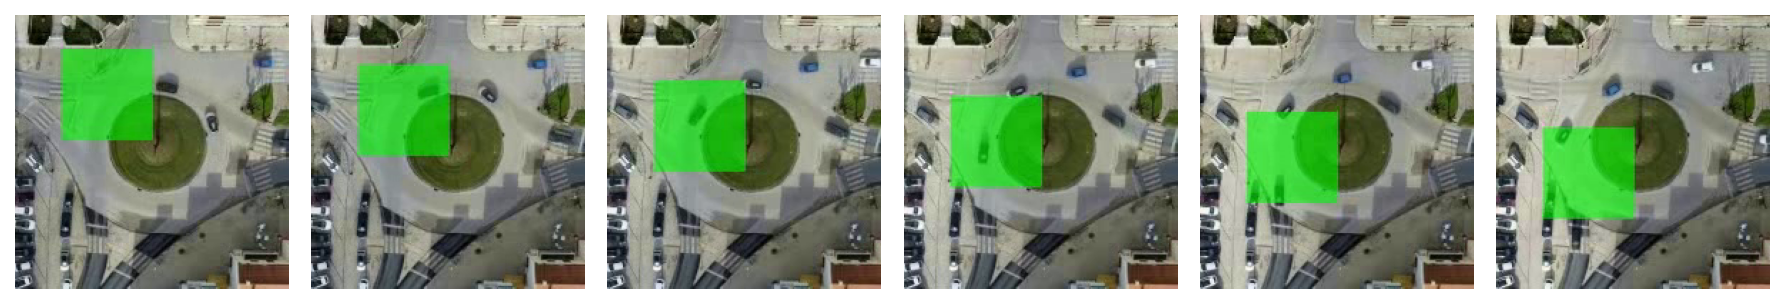
\includegraphics[width=\textwidth]{figures/13269_task_only.pdf}
\caption{An example inpainting task from our Traffic-Scenes dataset. }
\label{fig:semantics}
\end{figure*}
Further, prior work has overlooked the utility of the \emph{semantic} content of the video being inpainted, an understanding of which is particularly important for tasks where inpainting effectively amounts to inferring the behavior of occluded objects. To illustrate this, consider \cref{fig:semantics}. The black car at the top of the roundabout enters the masked region (shown in green) shortly after the first frame, and emerges some seconds later near the bottom of the frame. For an inpainting to be plausible, the car must follow a realistic trajectory around the roundabout. Note that, without a strong prior, there is insufficient information in the context to determine what such a trajectory might look like; the model must have some notion of what makes a vehicle trajectory plausible at a semantic level. For the roundabout example above, this includes, for instance, that vehicles should remain on the road surface, that vehicles travel forward with respect to their orientation, \etc. To accomplish this, the model must also correctly observe the entry and exit points of the vehicle, which could be arbitrarily far apart from each other in the general case. Additionally, the video inpainting problem is ill-posed -- given the events observed in the context, there exists a diversity of plausible trajectories the car could take, and video inpainting methods should account for this. As such, we assert that video inpainting methods must be capable of incorporating semantic knowledge, modeling long-range dependencies, and generating diverse solutions to solve the general video inpainting problem.

 
We argue that a sensible approach to video inpainting is to learn a conditional distribution over possible inpaintings given the observed context. Indeed, generative approaches to image inpainting using GANs \citep{imin3, imin4, imin5}, autoregressive models \citep{imin1}, and diffusion models \citep{palette, repaint} have long been amongst the top performing methods for image inpainting, and are capable of generating diverse, semantically coherent outputs. Such an approach has recently been made possible by the development of diffusion models for video \citep{didrik, fdm, vdm, yang2022diffusion, voleti2022MCVD}, which are capable of generating long, temporally coherent, photorealistic samples. In this work, we present a framework for using conditional video diffusion models for video inpainting. We demonstrate how to use long-range temporal attention to generate semantically consistent behaviour of inpainted objects over long time horizons, even when our model cannot be jointly model all frames due to memory constraints. We can do this even for inpainted objects that have limited or no visibility in the context, a quality not present in the current literature. We report strong experimental results on several challenging video inpainting tasks, outperforming state-of-the-art approaches on a range of standard metrics.

\begin{figure*}[h!]
    \centering
    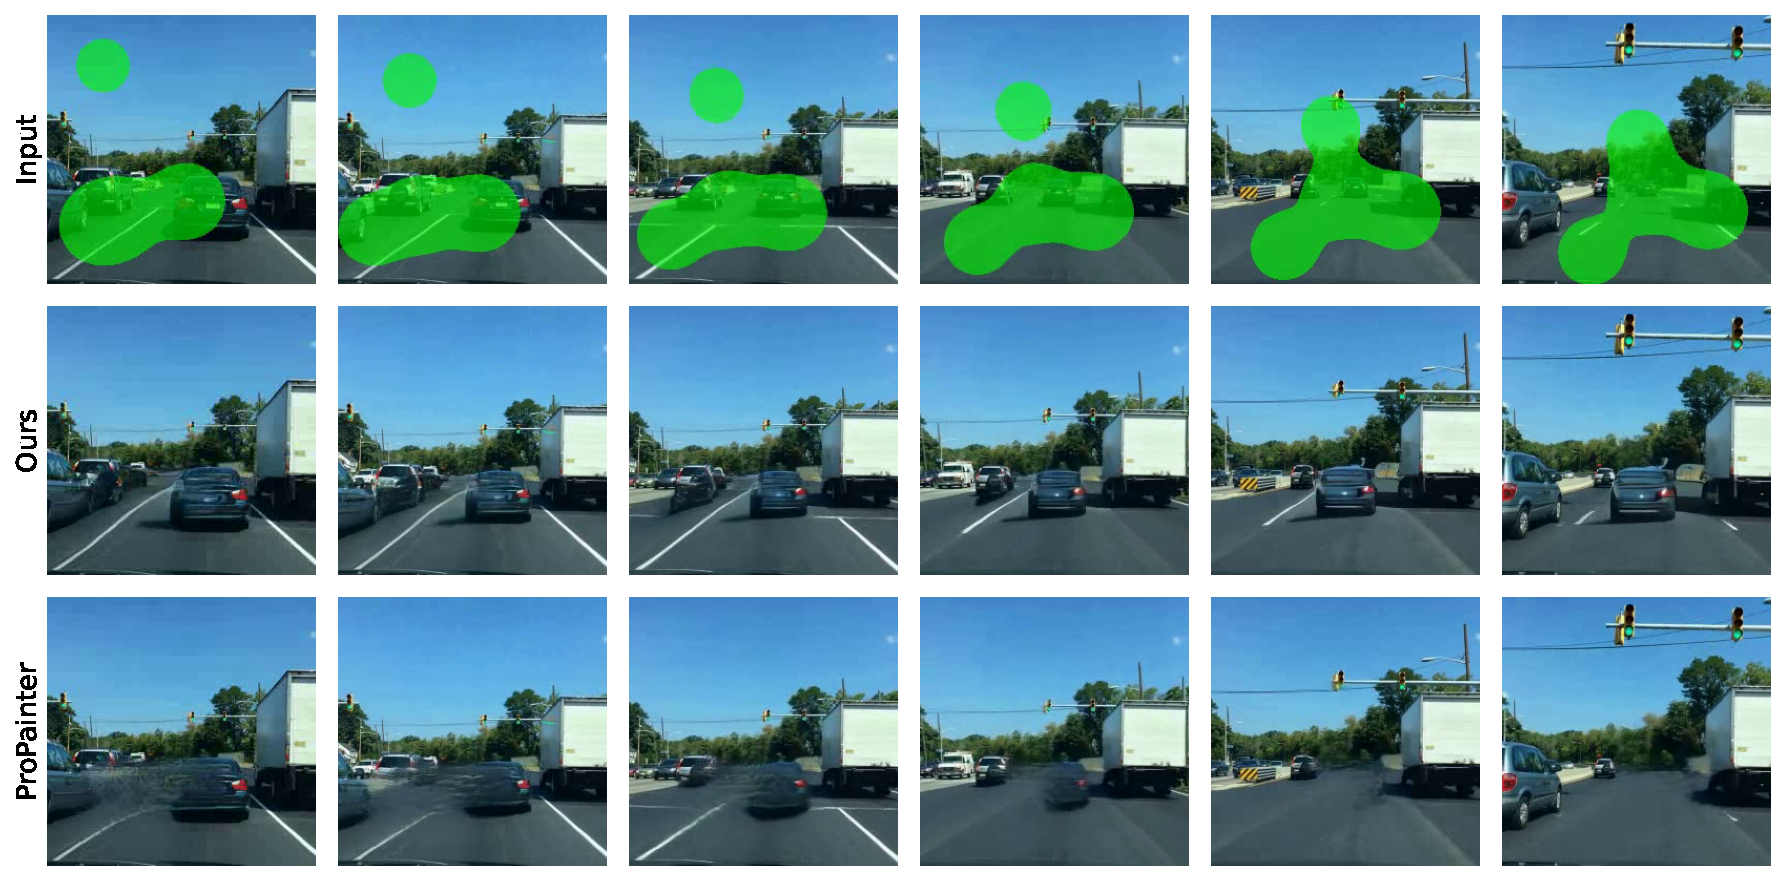
\includegraphics[width=\textwidth]{figures/bddv2.pdf}
    \caption{Inpainting results on a task from our BDD-Inpainting dataset. The first row shows the input to the model, with the occlusion mask marked in green. Our method (second row) is capable of generating a plausible completion of the partly occluded vehicle and realistically propagating it through time. On the contrary, in the result from the best-competing method, ProPainter \citep{propainter} (third row), the inpainted vehicle quickly fades away and is not modeled in a semantically consistent manner.}
    \label{fig:fig1}
\end{figure*}


\chapter{Preliminaries}
\section{Related Work}
\subsection{Video Inpainting} 
Recent advances in video inpainting have largely been driven by methods which fill in masked regions by borrowing content from the unmasked regions of other frames. These methods typically use optical flow estimates \citep{temporally, deepvideoinpainting, dfvi, flowedgeguided}, self-attention \citep{learningjoint, fuseformer, onionpeel, copypaste} or a combination of both \citep{propainter, fgt, endtoend} to determine how to propagate pixel values or learned features across frames. Such methods often produce visually compelling results, particularly on tasks where the mask-occluded region is visible in nearby frames such as foreground object removal. They struggle, however, in cases where this does not hold, for instance in the presence of heavy camera motion, large masks, or tasks where semantic understanding of the video content is required to produce a convincing result.

More recent work has utilized diffusion models for video inpainting. \citet{lookmanohands} uses a latent diffusion model \citep{stablediffusion, vahdat2021score} to remove the agent's view of itself from egocentric videos for applications in robotics. Notably, this is framed as an image inpainting task, where the goal is to remove the agent (with a mask provided by a segmentation model) from a single video frame conditioned on $h$ previous frames. Consequently, the results lack temporal consistency when viewed as videos, and the model is evaluated using image inpainting metrics only. \citet{avid} proposes a method for the related task of text-conditional video inpainting, which produces impressive results but requires user intervention. Most similar to this work, \citet{fgdvi} proposes a method for video inpainting that combines a video diffusion model with optical flow guidance. 


\subsection{Image Inpainting with Diffusion Models}
This work takes inspiration from the recent success of diffusion models for image inpainting. These methods can be split into two groups: those that inpaint using an unconditional diffusion model by making heuristic adjustments to the sampling procedure \citep{repaint, copaint}, and those that explicitly train a conditional diffusion model which, if sufficiently expressive and trained to optimality, enables exact sampling from the conditional distribution \citep{palette,zhang2023adding}. We follow the latter approach in this work.


\section{Background}
\subsection{Conditional Diffusion Models}
A conditional diffusion model \citep{tashiro2021csdi, ddpm, sohldickstein} is a generative model parameterized by a neural network trained to remove noise from data. The network is conditioned on $t \in \{ 1, \ldots, T\}$, an integer describing how much noise has been added to the data. Given hyperparameters $1 > \bar{\alpha}_1 > \ldots > \bar{\alpha}_T > 0$, training data is created by multiplying the original data by a factor $\sqrt{\bar{\alpha}_t}$ and then adding unit Gaussian noise $\boldsymbol{\epsilon}$ scaled to have variance $(1-\bar{\alpha}_t^2)$. The network should then map from this noisy data, the timestep $t$, and conditioning input $\mathbf{y}$, to a prediction of the added noise $\boldsymbol{\epsilon}$. It is trained with the squared error loss
\begin{equation}
    \mathcal{L}(\theta):=\mathbb{E}_{t, \mathbf{x}, \mathbf{y}, \boldsymbol{\epsilon}}\left[\left\|\boldsymbol{\epsilon}-\boldsymbol{\epsilon}_\theta\left(\sqrt{\bar{\alpha}_t} \mathbf{x}+\sqrt{1-\bar{\alpha}_t} \boldsymbol{\epsilon}, \mathbf{y}, t\right)\right\|^2\right],
    \label{eq:lsimple}
\end{equation}
where $\boldsymbol{\epsilon}_\theta(\ldots)$ is the output of the network. Data $\mathbf{x}$ and $\mathbf{y}$ are sampled from the data distribution $p_\text{data}$, and the timestep $t$ is typically sampled from a pre-specified categorical distribution. Once such a ``denoising'' network has been trained, various methods exist for using it to draw approximate samples from $p_\text{data}(\mathbf{x}|\mathbf{y})$ \citep{ddpm,sohldickstein,tashiro2021csdi,song2020score,karras2022elucidating}. We use the Heun sampler proposed by \citet{karras2022elucidating}, and leave further details to the appendix.

\begin{figure}[t]
    \centering
    \begin{subfigure}[t]{0.3\textwidth}
        \centering
        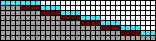
\includegraphics[width=\textwidth]{figures/sampling-scheme-visualizations/autoreg.png}
        \caption{AR}
        \label{fig:ar}
    \end{subfigure}
    ~
    \begin{subfigure}[t]{0.3\textwidth}
        \centering
        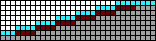
\includegraphics[width=\textwidth]{figures/sampling-scheme-visualizations/reverse-autoreg.png}
        \caption{Reverse AR}
        \label{fig:rev_ar}
    \end{subfigure}
    ~
    \begin{subfigure}[t]{0.3\textwidth}
        \centering
        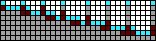
\includegraphics[width=\textwidth]{figures/sampling-scheme-visualizations/hierarchy-2.png}
        \caption{Hierarchy-2}
        \label{fig:h2}
    \end{subfigure}
    \caption[A visualization of sampling schemes introduced in prior work.]{A visualization of sampling schemes (introduced in \citet{fdm}) for generating videos of length $N=31$ while accessing only $K=8$ frames at a time. Each row of each subfigure depicts a different stage of our sampling process, starting from the top row and working down. Each column represents one video frame. Within each stage, frames shown in \textcolor{latentcolor}{cyan} are being sampled conditioned on the values of previously-sampled frames shown in \textcolor{observedpastcolor}{dark red}. Frames shown in white are not yet generated. By the end, all frames are generated and shown in \textcolor{completecolor}{light gray}.
    }
    \label{fig:old-sampling-schemes}
\end{figure}


\subsection{Video Diffusion Models}
Before we discuss conditional video diffusion models, we first discuss video diffusion models in general. A number of recent papers have proposed diffusion-based approaches to generative modeling of video data \citep{didrik, fdm, vdm, yang2022diffusion, voleti2022MCVD}. 
We follow the majority of these approaches \citep{fdm,vdm,voleti2022MCVD} in using a 4-D U-Net~\citep{unet} architecture to parameterize $\boldsymbol{\epsilon}_\theta(\ldots)$. 
Alternating spatial and temporal attention blocks within the U-Net capture dependencies within and across frames respectively, with relative positional encodings \citep{rpe1, rpe2} providing information about each frame's position within the video. 
Due to computational constraints, video diffusion models are inherently limited to conditioning on and generating a small number of frames at a time, which we denote as $K$. 

\subsection{Flexible Video Diffusion Models}
Generating long videos with numbers of frames $N \gg K$ then requires sampling from the diffusion model multiple times. A typical approach would be to break the generation down into multiple stages, and in each stage sample $K/2$ frames conditioned on the previous $K/2$ frames. 
We depict this approach in \Cref{fig:ar}, with each row representing one stage. A problem with this strategy is that it fails to capture dependencies on frames more than $K/2$ frames in the past. 
Alternative orders in which to generate frames (which we will refer to as ``sampling schemes'') are possible, with some additional ones depicted in \Cref{fig:h2,fig:rev_ar}. Each of these sampling schemes tends to have its downsides, and experimentation usually requires expensive retraining of models. 
\citet{fdm} therefore suggest training a single model that can perform well on any sampling scheme. In particular, they train a model to generate any subset of video frames conditioned on any other subset with the objective
\begin{equation}
    \mathcal{L}_{\text {flexible}}(\theta):=\mathbb{E}_{t, \mathbf{x}, \mathbf{y}, \mathcal{X}, \mathcal{Y}, \boldsymbol{\epsilon}}\left[\left\|\boldsymbol{\epsilon}-\boldsymbol{\epsilon}_\theta\left(\sqrt{\bar{\alpha}_t} \mathbf{x}+\sqrt{1-\bar{\alpha}_t} \boldsymbol{\epsilon}, \mathbf{y}, \mathcal{X}, \mathcal{Y}, t\right)\right\|^2\right],
    \label{eq:lflexible}
\end{equation}
in which $\mathbf{x}$ are the frames to remove noise from at indices $\mathcal{X}$, and $\mathbf{y}$ are the frames to condition on at indices $\mathcal{Y}$. 
To sample $\mathbf{x}$ and $\mathbf{y}$ we first sample $\mathcal{X}$ and $\mathcal{Y}$, then sample a training video, and then extract the frames at indices $\mathcal{X}$ and $\mathcal{Y}$ to form $\mathbf{x}$ and $\mathbf{y}$, respectively.
Both the number of frames to generate and the number to condition on can vary, so the shapes of $\mathbf{x}$, $\boldsymbol{\epsilon}$, and $\mathbf{y}$ can vary correspondingly. The network is given the indices of all frames ($\mathcal{X}$ and $\mathcal{Y}$), as they are used to create the relative positional encodings \citep{rpe1, rpe2}. 
Once a network is trained to make predictions for arbitrary indices $\mathcal{X}$ given arbitrary indices $\mathcal{Y}$, it can be used to sample long videos with any desired sampling scheme. Sampling schemes will henceforth be denoted as $\{\mathcal{X}_s, \mathcal{Y}_s\}_{s=1}^S$ where $S$ is the number of sampling stages and, at stage $s$, $\mathcal{X}_s$ and $\mathcal{Y}_s$ are the indices of the latent and observed frames, respectively. 











 
\chapter{Method}
\label{sec:VICDM}

\begin{figure}[t]
    \centering
        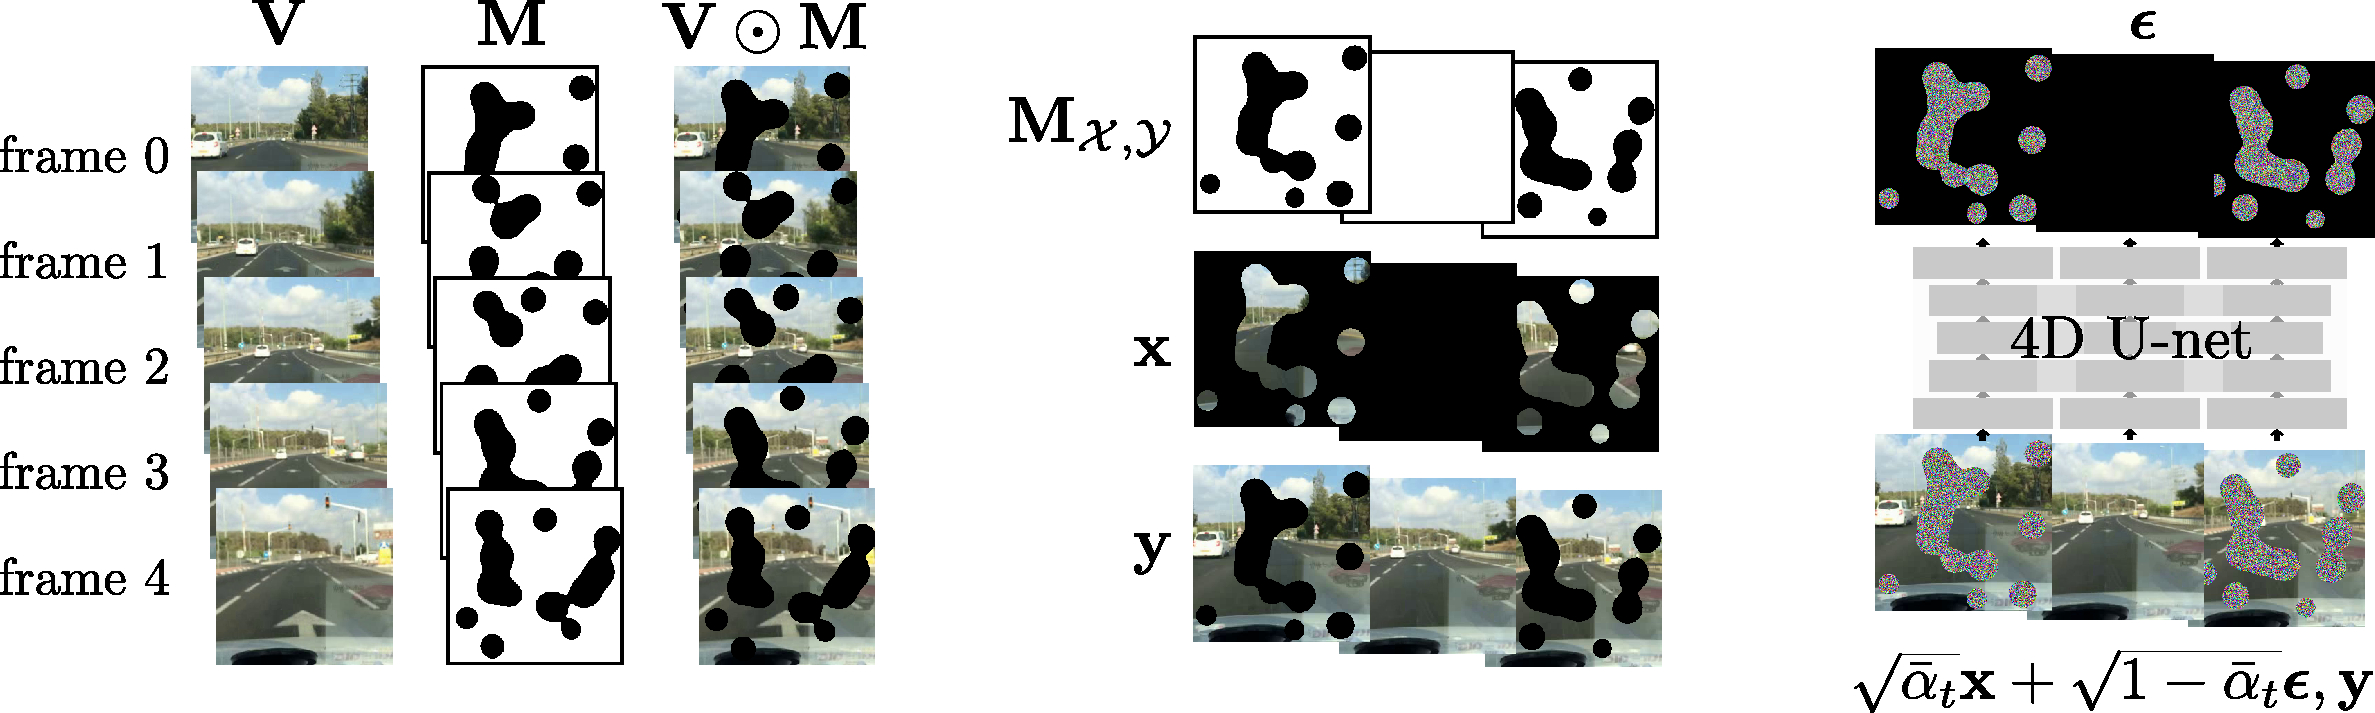
\includegraphics[width=0.9\textwidth]{figures/architecture-overview/video-inpainting-overview.pdf}
    \caption[Example model inputs during training.]{Example model inputs during training. \textbf{Left:} Visualizations of a 5-frame video $\bV$, a corresponding mask $\bM$, and the resulting known pixel values $\bV\odot\bM$. \textbf{Center:} Collated training inputs if $\fX = [0, 3]$ and $\fY = [2]$. The observations in $\by$ are then the whole of frame 2 and known pixel values in frames 0 and 3. The task is to predict the unknown pixel values in frames 0 and 3. \textbf{Right:} Inputs fed to the neural network, with noise added to pixel values in $\mathbf{x}$ but not those in $\mathbf{y}$. The task is then to predict the noise $\epsilon$. For simplicity we do not show inputs $t$, $\bM_{\fX,\fY}$, or $\fX\oplus\fY$.}
    \label{fig:arch-and-training}
\end{figure}

\section{Problem Formulation}
% \defeq \left[\bv_i\right]^N_{i=1}$,
% \defeq \left[\bm_i\right]^N_{i=1}$
We consider the problem of creating an $N$-frame video $\bV$ conditioned on some subset of known pixel values specified by a pixel-level mask $\bM$. Entries of $\bM$ take value $1$ where the corresponding pixel in $\bV$ is known and take $0$ elsewhere. We frame this as a conditional generative modeling problem, where we aim to learn an approximation of the posterior under the data distribution $p_\theta(\bV|\bV \odot \bM) \approx p_\text{data}(\bV|\bV \odot \bM)$, with $\odot$ defined such that $a \odot \bM$ returns the set of elements in $a$ for which the corresponding value in $\bM$ is 1.


Recall that, due to constraints from the network architecture, \citet{fdm} were restricted to conditioning on or generating at most $K$ frames at a time. In the video inpainting problem we are predicting and conditioning on pixels rather than frames, but our network architecture imposes an analogous constraint: we can only predict or condition on pixels from at most $K$ different frames at a time. We modify the definition of a sampling scheme from \citet{fdm} as follows: we again denote sampling schemes $\{\mathcal{X}_s, \mathcal{Y}_s\}_{s=1}^S$ with $\mathcal{X}_s$ and $\mathcal{Y}_s$ being collections of frame indices. Now, however, at each stage we sample values for only unknown pixels in frames indexed by $\mathcal{X}_s$, and condition on known pixel values in all frames indexed by either $\mathcal{X}_s$ or $\mathcal{Y}_s$. Referencing \Cref{fig:sampling-schemes}, in each row (stage) we show frames indexed by $\mathcal{X}_s$ in cyan and frames indexed by $\mathcal{Y}_s$ in either dark red or bright red. Frames shown in bright red contain missing pixels, which we do not wish to sample or condition on until a later sampling stage; we describe how we deal with this in \Cref{sec:future-conditioning}.


\section{Architecture}
We generalize the FDM architecture of \citet{fdm} to use pixel-level masks rather than frame-level masks, as in the image inpainting approach proposed by \citet{palette}. Concretely, every input frame is concatenated with a mask which takes value $1$ where the corresponding pixel is observed and $0$ elsewhere. The input values are clean (without added noise) for observed pixels and noisy values otherwise.



\section{Training Procedure} 
Recall that we wish to train a model that can generate plausible values for unknown pixels in frames indexed by $\mathcal{X}$, conditioned on known pixel values in frames indexed by either $\mathcal{X}$ or $\mathcal{Y}$. We simulate such tasks by first sampling a video $\bV$ and a mask $\bM$ from our dataset,  and then sampling frame indices $\mathcal{X}$ and $\mathcal{Y}$ from a ``frame index distribution'' similar to that of \citet{fdm}.\footnote{Our frame index distribution is a mixture distribution between the one used by \citet{fdm} and one which always samples $\mathcal{X}$ and $\mathcal{Y}$ so that they represent sequences of consecutive frames. We found that including these sequences of consecutive frames improved temporal coherence.}
The distribution over masks $\bM$ can be understood as reflecting the variability in the types of masks we will encounter at test-time, and the frame index distribution can be understood as reflecting our desire to be able to sample from the model using arbitrary sampling schemes. Given $\bM$, $\fX$, and $\fY$, we create a combined list of frames $\fX \oplus \fY$, where $\oplus$ denotes concatenation, and a corresponding mask $\bM_{\fX,\fY} := \bM[\fX] \oplus \mathbbm{1}[\fY]$, where $\mathbbm{1}[\mathcal{Y}]$ is a mask of all $1$'s for each frame indexed in $\mathcal{Y}$. This masks only the missing pixels in frames $\fX$ while treating all pixels in frames $\fY$ as observed (visualized in \Cref{fig:arch-and-training}).
We then extract our training targets from the video as $\bx := \bV[\fX\oplus\fY] \odot (1-\bM_{\fX,\fY})$, and our observations as $\by := \bV[\fX\oplus\fY] \odot \bM_{\fX,\fY}$.

\begin{algorithm}[t]
    \caption{Training Loop}
    \label{alg:train}
    \begin{algorithmic}[1]
    \Repeat
    \State $(\bV, \bM) \sim q(\bV, \bM)$\Comment{Sample video and mask}
    \State $(\mathcal{X}, \mathcal{Y}) \sim u(\mathcal{X}, \mathcal{Y})$\Comment{Sample training task}
    \State $t \sim \mathcal{U}(\{1 \ldots T\})$\Comment{Sample timestep}
    \State $\boldsymbol{\epsilon} \sim \mathcal{N}(\mathbf{0}, \mathbf{I})$\Comment{Sample noise}
    \State $\bM_{\mathcal{X}, \mathcal{Y}} \gets \bM [\mathcal{X}] \oplus \mathbbm{1}[\fY]$\Comment{Create training mask}
    \State $\bx \gets \bV[\fX \oplus \fY] \odot (\mathbf{1} - \bM_{\fX, \fY})$\Comment{Extract noised pixels} 
    \State $\by \gets \bV[\fX \oplus \fY] \odot \bM_{\fX, \fY}$\Comment{Extract known pixels} 
    \State Compute $\mathcal{L}_{\text{ours}}(\theta)$ and take gradient descent step\Comment{See \Cref{eq:lours}}
    \Until converged
\end{algorithmic}
\end{algorithm}

Resampling $\bV$, $\bM$, $\fX$, and $\fY$ for every training example therefore defines a distribution over $\bx$ and $\by$, which we use when estimating the expectation over them in \Cref{eq:lflexible}. Combining this method of sampling $\bx$ and $\by$ with our pixel-wise mask, we write the loss as
\begin{equation}
    \mathcal{L}_{\text{ours}}(\theta):=\mathbb{E}_{t, \mathbf{x}, \mathbf{y}, \mathcal{X}, \mathcal{Y}, \boldsymbol{\epsilon}}\left[(\mathbf{1}-\bM_{\fX,\fY})\odot\left\|\boldsymbol{\epsilon}-\boldsymbol{\epsilon}_\theta\left(\sqrt{\bar{\alpha}_t} \mathbf{x}+\sqrt{1-\bar{\alpha}_t} \boldsymbol{\epsilon}, \mathbf{y}, \bM_{\fX,\fY}, \fX\oplus\fY, t\right)\right\|^2\right],
    \label{eq:lours}
\end{equation}
where $\fX\oplus\fY$ provides information about each frame's index within $\bV$, and $\bM_{\fX,\fY}$ is the mask making explicit which pixels have known values.We note that the loss is only computed for unknown pixel locations. The full training loop is outlined in \Cref{alg:train}.




\section{Inpainting Long Videos} \label{sec:future-conditioning}
Given the architecture and training procedure we have described so far, we can use the resulting models to to implement the AR and Hierarchy-2 sampling schemes shown in \Cref{fig:ar,fig:h2} without further complication. A downside of these sampling schemes, however, is that they do not enable us to condition on frames with unknown pixel values. That is, we are not able to condition on the known pixels in a frame unless we either (a) have previously inpainted it and know all of its pixel values already, or (b) are inpainting it as we condition on it. We show in our experiments that this often leaves us unable to account for important dependencies in the context.



We therefore propose a method for conditioning on \textit{incomplete} frames. This enables the sampling schemes shown in \Cref{fig:sampling-schemes}, where we condition on the known pixels in incomplete frames, marked in red. Recall that $\bx$ denotes ``unknown pixels in frames indexed by $\fX$'' and $\by$ denotes ``known pixels in frames indexed by $\fX$ or $\fY$''. If any frames indexed by $\fY$ are incomplete then we have a third category, which we'll call $\mathbf{z}$: ``unknown pixels in frames indexed by $\fY$''.




We then wish to approximately sample $\mathbf{x} \sim p_\text{data}(\cdot | \mathbf{y})$ without requiring values of $\mathbf{z}$. We do not have a way to sample directly from an approximation of this distribution, as the diffusion model is not trained to condition on ``incomplete'' frames. We note, however, that this desired distribution is the marginal of a distribution that our diffusion model \textit{can} approximate:
\begin{equation}
    p_\text{data}(\mathbf{x}|\mathbf{y}) = \int p_\text{data}(\mathbf{x},\mathbf{z}|\mathbf{y}) \mathrm{d}\mathbf{z} \approx \int p_\theta(\mathbf{x},\mathbf{z}|\mathbf{y}) \mathrm{d}\mathbf{z}.
\end{equation}
This means that we can sample from the required approximation of $p_\text{data}(\mathbf{x}|\mathbf{y})$ by sampling from $p_\theta(\mathbf{x},\mathbf{z}|\mathbf{y})$ and then simply discarding $\mathbf{z}$.

\begin{figure}[t]
    \centering
    \begin{subfigure}[t]{0.3\textwidth}
        \centering
        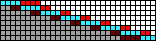
\includegraphics[width=\textwidth]{figures/sampling-scheme-visualizations/autoregressive-with-near-future.png}
        \caption{Improved AR.}
        \label{fig:improved-ar}
    \end{subfigure}
    ~
    \begin{subfigure}[t]{0.3\textwidth}
        \centering
        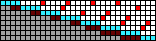
\includegraphics[width=\textwidth]{figures/sampling-scheme-visualizations/autoregressive-with-future.png}
        \caption{Improved AR w/ \\ far future.}
        \label{fig:improved-ar-w-far-future}
    \end{subfigure}
    ~
    \begin{subfigure}[t]{0.3\textwidth}
        \centering
        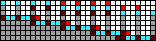
\includegraphics[width=\textwidth]{figures/sampling-scheme-visualizations/autoregressive-multires-3-1.png}
        \caption{2-res. improved AR.}
        \label{fig:multiscale}
    \end{subfigure}%
    \caption[A visualization of sampling schemes for video inpainting.]{Sampling schemes visualizations similar to \Cref{fig:old-sampling-schemes}. In addition we now also condition on observed pixel values in frames that can also contain unknown pixel values. Frames where we do so are shown in bright red and the color scheme is otherwise the same as in \Cref{fig:old-sampling-schemes}.
    }
    \label{fig:sampling-schemes}
\end{figure}

\section{Sampling Schemes}\label{sec:samplingschemes}
The ability to condition on incomplete frames enables us to design new sampling schemes that better capture dependencies that are necessary for high-quality video inpainting. \textbf{Improved AR} is a variant of AR that takes into account information from future frames by conditioning on the observed parts of the frames immediately after the sequence of frames being generated, as well as on the frames before; see \Cref{fig:improved-ar}. \textbf{Improved AR w/ Far Future} builds on ``Improved AR'' by conditioning on the observed parts of frames far in the future instead of of frames immediately after those being sampled; see \Cref{fig:improved-ar-w-far-future}.
\textbf{3-Resolution Improved AR} (3-Res. Improved AR) builds on ``Improved AR'' by first infilling every fifteenth frame using Improved AR, then infilling every fifth frame while conditioning on nearby infilled frames, and then infilling all other frames. We visualize a ``2-res.'' version (infilling every third frame and then every frame) in \Cref{fig:multiscale}. Visualizations of all sampling schemes we consider are shown in \Cref{fig:sampling-scheme-details}. 

\begin{figure}[t!]
    \centering
    \begin{subfigure}[t]{\textwidth}
        \centering
        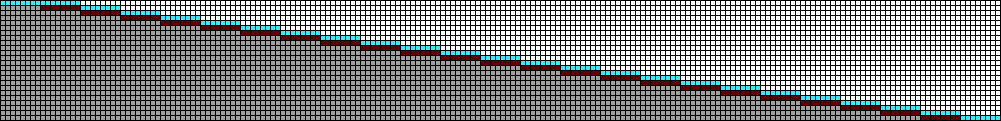
\includegraphics[width=\textwidth]{figures/big-sampling-scheme-visualizations/autoreg.png}
        \caption{AR.}
        \label{fig:ar-app}
    \end{subfigure}
    ~
    \begin{subfigure}[t]{\textwidth}
        \centering
        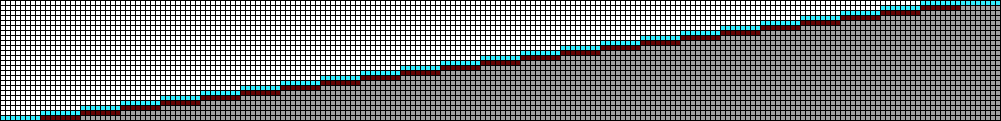
\includegraphics[width=\textwidth]{figures/big-sampling-scheme-visualizations/reverse-autoreg.png}
        \caption{Reverse AR.}
        \label{fig:reverse-ar-app}
    \end{subfigure}
    ~
    \begin{subfigure}[t]{\textwidth}
        \centering
        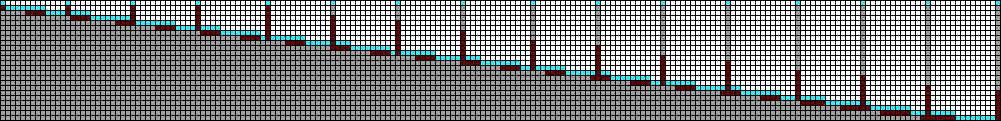
\includegraphics[width=\textwidth]{figures/big-sampling-scheme-visualizations/hierarchy-2.png}
        \caption{Hierarchy-2.}
        \label{fig:h2-app}
    \end{subfigure}
    ~
    \begin{subfigure}[t]{\textwidth}
        \centering
        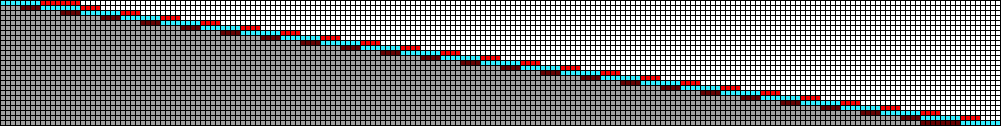
\includegraphics[width=\textwidth]{figures/big-sampling-scheme-visualizations/autoregressive-with-near-future.png}
        \caption{Improved AR.}
        \label{fig:improved-ar-app}
    \end{subfigure}
    ~
    \begin{subfigure}[t]{\textwidth}
        \centering
        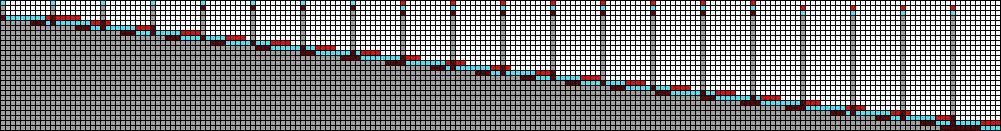
\includegraphics[width=\textwidth]{figures/big-sampling-scheme-visualizations/autoregressive-multires-10-1.png}
        \caption{2-Res Improved AR.}
        \label{fig:2res-app}
    \end{subfigure}
    ~
    \begin{subfigure}[t]{\textwidth}
        \centering
        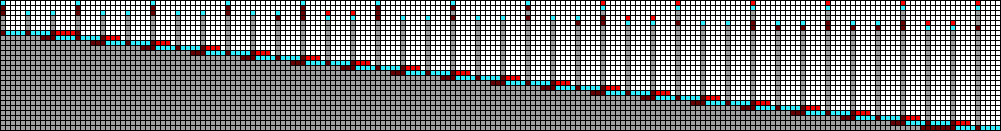
\includegraphics[width=\textwidth]{figures/big-sampling-scheme-visualizations/autoregressive-multires-15-5-1.png}
        \caption{3-Res Improved AR.}
        \label{fig:3res-app}
    \end{subfigure}
    ~
    \begin{subfigure}[t]{\textwidth}
        \centering
        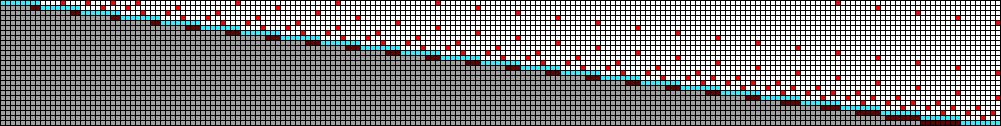
\includegraphics[width=\textwidth]{figures/big-sampling-scheme-visualizations/autoregressive-with-future.png}
        \caption{Improved AR with Far Future.}
    \end{subfigure}
    \caption[A visualization of all sampling schemes.]{Sampling schemes visualizations similar to \Cref{fig:old-sampling-schemes}, but with a model capable of attending to 16 frames at a time as in our experiments, and a more typical video length of 200.
    }
    \label{fig:sampling-scheme-details}
\end{figure}

\begin{comment}
\begin{minipage}{0.46\textwidth}
\begin{algorithm}[H]
    \centering
    \caption{Example Algorithm}\label{algorithm}
    \begin{algorithmic}[1]
\Repeat
\State $(\bV, \bM) \sim q(\bV, \bM)$\Comment{Sample video and mask}
\State $(\mathcal{X}, \mathcal{Y}) \sim u(\mathcal{X}, \mathcal{Y})$\Comment{Sample training task}
\State $t \sim \mathcal{U}(\{1 \ldots T\})$
\State $\boldsymbol{\epsilon} \sim \mathcal{N}(\mathbf{0}, \mathbf{I})$
\State $(\bV', \bM') \gets (\bV[\fX \cup \fY], \bM[\fX \cup \fY])$
\State $\bV_t' \gets \sqrt{\bar{\alpha}_t}\bV' + \sqrt{1-\bar{\alpha}_t}(\mathbbm{1}-\bM')\odot\boldsymbol{\epsilon}$
\State Take gradient descent step on \newline 
\hspace*{5em}$\nabla_\theta \|(1-\bM')\odot(\boldsymbol{\epsilon} - \boldsymbol{\epsilon}_\theta(\bV_t', \bM', \mathcal{X}, \mathcal{Y}, t))\|^2$
\Until converged
    \end{algorithmic}
\end{algorithm}
\end{minipage}
\hfill
\begin{minipage}{0.46\textwidth}
\begin{algorithm}[H]
    \centering
    \caption{Example Algorithm}\label{algorithm1}
    \begin{algorithmic}[1]
\For{$s \gets 1, \ldots, S$}
\State $\bV_s \gets \bV [\fX_s \cup \fY_s]$\Comment{Extract video frames}
\State $\bM_s \gets \bM [\fX_s \cup \fY_s]$\Comment{Extract mask frames}
\State $\hat{\bV}_s \sim \texttt{DDPM}(\cdot;\bV_s, \bM_s, \theta)$\Comment{Sample}
\State $\bV [\fX_s \cup \fY_s] \gets \hat{\bV}_s$\Comment{Insert completed frames}
\State $\bM [\fX_s] \gets \mathbbm{1}$\Comment{Update masks for inpainted frames}
\EndFor
\State \Return $\bV$
    \end{algorithmic}
\end{algorithm}
\end{minipage}


\begin{algorithm}[t]
\caption{Inpaint a video $\bV$ given binary mask $\bM$ and sampling scheme $\left[(\mathcal{X}_s, \mathcal{Y}_s)\right]^S_{s=1}$}
\label{alg:alg}
\begin{algorithmic}[1]
\Procedure{InpaintVideo}{$\bV, \bM; \theta$}
\For{$s \gets 1, \ldots, S$}
\State $\bV_s \gets \bV [\fX_s \cup \fY_s]$\Comment{Extract video frames}
\State $\bM_s \gets \bM [\fX_s \cup \fY_s]$\Comment{Extract mask frames}
\State $\hat{\bV}_s \sim \texttt{DDPM}(\cdot;\bV_s, \bM_s, \theta)$\Comment{Sample}
\State $\bV [\fX_s \cup \fY_s] \gets \hat{\bV}_s$\Comment{Insert completed frames}
\State $\bM [\fX_s] \gets \mathbbm{1}$\Comment{Update masks for inpainted frames}
\EndFor
\State \Return $\bV$
\EndProcedure
\end{algorithmic}
\end{algorithm}
\end{comment}


\chapter{Experiments}
\section{Datasets}
To highlight the unique capabilities our generative approach offers, we wish to target video inpainting tasks in which visual information in nearby frames cannot be easily exploited to achieve a convincing result. The YouTube-VOS \citep{youtubevos1} (training and test) and DAVIS \citep{davis} (test) video object segmentation datasets have become the \emph{de facto} standard benchmark datasets for video inpainting in recent years, and the foreground object masks included in these datasets have led to a heavy focus on object removal tasks in qualitative evaluations of video inpainting methods. Object removal in these datasets is a task to which \eg optical flow-based approaches are specifically well suited, as the backgrounds are often near-stationary and so information in neighboring frames can be used to great effect. In contrast, we wish to focus on tasks where inpainting requires the visual appearances of objects to be hallucinated in whole or in part and realistically propagated through time, or where the behavior of occluded objects must be inferred. We propose four new large-scale video inpainting datasets targeting such tasks. All datasets are 256 $\times$ 256 resolution and 10 fps. Representative examples of each dataset, along with details of how each dataset was constructed, are included in \cref{app:datasetss}.
%Additionally, the YouTube-VOS training set is problematic for training with our generative approach, as the videos are semantically diverse and the scale of the dataset is small \hlk{(3471 videos containing $\sim$200 frames each)} relative to datasets typically used to train video generative models.
\begin{figure*}[t]
\centering
\includegraphics[width=\linewidth]{figures/13269_shaded_cropped.pdf}
\caption{Inpaintings from our model and ProPainter on the task introduced in \cref{fig:semantics} from our Traffic-Scenes dataset. Our model can inpaint a realistic trajectory for the occluded vehicle. Competing flow-based approaches correctly inpaint the background but are unable to account for the vehicle.}
\label{fig:traffic-scenes}
\end{figure*}
\begin{figure*}[t]
\centering
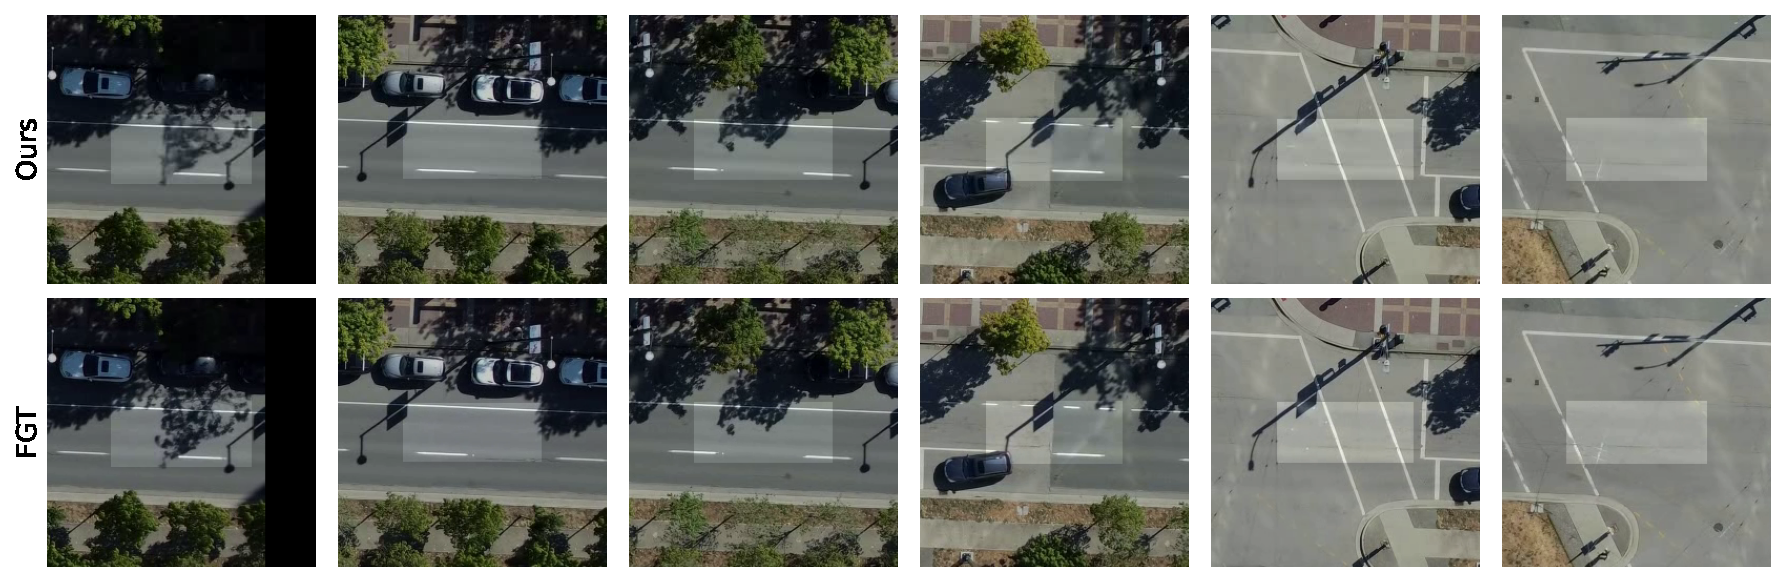
\includegraphics[width=\linewidth]{figures/bg_3119.pdf}
\caption{Inpainted videos from our Inpainting-Background dataset. Results from our method are displayed on the top row; results from the best competing model FGT \citep{fgt} are on the bottom row. The ground truth region is darkened slightly to aid in visualizing the boundary between generated and ground-truth regions. Despite FGT outperforming our method on quantitative metrics, qualitative results are similar in quality.}
\label{fig:background}
\end{figure*}
\subsection{BDD-Inpainting}
We adapt the BDD100K \citep{bdd100k} dataset for the video inpainting task. This dataset contains 100,000 high-quality first-person driving videos and includes a diversity of geographic locations and weather conditions. We select a random subset of approximately 50,000 
of these, and generate a set of both moving and stationary masks of four types: grids, horizontal or vertical lines, boxes (\cref{fig:traffic-scenes}), and blobs (\cref{fig:fig1}). During training both videos and masks are sampled uniformly, giving a distribution over an extremely varied set of inpainting tasks. We include two test sets of 100 video-mask pairs each, the first (BDD-Inpainting) containing only grid, line, and box masks, and the second (BDD-Inpainting-Blobs) containing only blob masks. The second is a substantially more challenging test set, as the masks are often large and occlude objects in the scene for a significant period of time. See the appendix for representative examples. The test sets we use, along with code for processing the original BDD100K dataset and generating masks, will be released upon publication. 
\subsection{Inpainting-Cars and Inpainting-Background}
We use an in-house dataset of overhead drone footage of vehicle traffic, for which we have tracker-generated bounding boxes for each vehicle, to create two task-specific datasets. The first, Inpainting-Background (\cref{fig:background}), targets the removal of cars from videos by using time-shifted bounding boxes as occlusion masks, where the bounding boxes are shifted such that the masked-out region contains only the road surface and other environmental factors. The second, Inpainting-Cars (\cref{fig:cars}), targets the \emph{addition} of cars to videos by using the original bounding boxes as masks so that the masked-out region always contains a single vehicle. Note that the masked-out vehicle is not visible at any time in the context, and so,  given an input, the model must hallucinate a vehicle and propagate it through time, using only the size and movement of the mask as clues to plausible vehicle appearance and motion.
\subsection{Traffic Scenes}
Using the same in-house dataset as referenced above, we generate another dataset where large sections of the roadway are occluded, requiring the model to infer vehicle behavior in the masked-out region. Crops are centered over road features like intersections, roundabouts, highway on-ramps, \etc where complex vehicle behavior and interactions take place. This dataset contains exceptionally challenging video inpainting tasks as vehicles are often occluded for long durations of time, requiring the model to generate plausible trajectories that are semantically consistent with both the observations (e.g. the entry and exit point of a vehicle from the masked region) and the roadway. This dataset contains approximately 13,000 videos in the training set and 100 video-mask pairs in the test set. 
\section{Baselines and Metrics} 
We compare our method with four recently proposed video inpainting methods that achieve state-of-the-art performance on standard benchmarks: ProPainter \citep{propainter}, E$^2$FGVI \citep{endtoend}, FGT \citep{fgt}, and FGVC \citep{flowedgeguided}. For each model, we use pre-trained checkpoints made available by the respective authors. We adopt the evaluation suite of DEVIL \citep{devil}, which includes a comprehensive selection of commonly used metrics targeting three different aspects of inpainting quality:
\begin{itemize}
    \item Reconstruction, or how well the method's output matches the ground truth: PSNR, SSIM \citep{ssim}, LPIPS \citep{lpips}, PVCS \citep{devil}. 
    \item Perceptual realism, or how well the appearance and/or motion resembles a reference set of ground truth videos: FID \citep{fid}, VFID \citep{vfid}.
    \item Temporal consistency: Flow warping error ($E_\text{warp}$) \citep{ewarp}, which measures how well an inpainting follows the optical flow as calculated on the ground truth. 
\end{itemize} 
For our method, we train one model on each dataset with $K=16$. Models are trained on 4$\times$ NVIDIA A100 GPUs for 1-4 weeks. A detailed accounting of each model's hyperparameters and training procedure can be found in the appendix.



\begin{table}[t]
\centering
\caption[Quantitative comparison with state-of-the-art video inpainting methods across each of our four datasets.]{Quantitative comparison with state-of-the-art video inpainting methods across each of our four datasets. For each dataset/metric, the best performing model is indicated with bold font and the second best performing model is underlined. Improved AR w/ Far Future is used for all datasets but Inpainting-Background, which uses AR.}
\label{table:main}
\customrescaleone{

\begin{tabular}{llllllll}
\toprule
Method & PSNR$\blacktriangle$ & SSIM$\blacktriangle$   & LPIPS$\blacktriangledown$     & PVCS$\blacktriangledown$   & FID$\blacktriangledown$   & VFID$\blacktriangledown$   & $E_\text{warp}$$\blacktriangledown$ \\ 
\midrule
\multicolumn{8}{c}{BDD-Inpainting} \\
\midrule
ProPainter                       & \hlk{\underline{32.65}}  & \hlk{\underline{0.968}} & \hlk{\underline{0.0355}} & \hlk{\underline{0.2806}} & \hlk{\underline{2.51}}  & \hlk{\underline{0.1599}} & \hlk{$\mathbf{\,1.5{\cdot}10^{\shortminus3}}$}            \\
FGT                              & \hlk{28.50}  & \hlk{0.928} & \hlk{0.0843} & \hlk{0.6430} & \hlk{9.94}  & \hlk{0.7863} & \hlk{$\,4.0{\cdot}10^{\shortminus3}$}          \\
E$^2$FGVI                        & \hlk{30.16}  & \hlk{0.946} & \hlk{0.0640} & \hlk{0.4765} & \hlk{6.58}  & \hlk{0.3665} & \hlk{$\,2.3{\cdot}10^{\shortminus3}$}            \\
FGVC                             & \hlk{25.84}  & \hlk{0.884} & \hlk{0.1498} & \hlk{1.0210} & \hlk{32.08} & \hlk{1.7995} & \hlk{$\,7.5{\cdot}10^{\shortminus3}$}     \\
Ours                             & \hlbf{33.68}	& \hlbf{0.972} & \hlbf{0.0261} & \hlbf{0.2037}	& \hlbf{1.71}  & \hlbf{0.0748} & \hlk{\,$\underline{1.8{\cdot}10^{\shortminus3}}$} \\
\midrule
\multicolumn{8}{c}{BDD-Inpainting-Blobs} \\
\midrule
ProPainter                       & \hlk{\underline{30.54}}  & \hlk{\underline{0.960}} & \hlk{\underline{0.0467}} & \hlk{\underline{0.3120}} & \hlk{\underline{2.56}}  & \hlk{\underline{0.1499}} & \hlk{$\mathbf{\,1.2{\cdot}10^{\shortminus3}}$}               \\
FGT                              & \hlk{27.33}  & \hlk{0.938} & \hlk{0.0737} & \hlk{0.5130} & \hlk{9.41}  & \hlk{0.3594} & \hlk{$\,2.5{\cdot}10^{\shortminus3}$}            \\
E$^2$FGVI                        & \hlk{29.04}  & \hlk{0.950} & \hlk{0.0667} & \hlk{0.4414} & \hlk{4.23}  & \hlk{0.2339} & \hlk{$\,1.7{\cdot}10^{\shortminus3}$}            \\
FGVC                             & \hlk{25.10}  & \hlk{0.913} & \hlk{0.0980} & \hlk{0.6957} & \hlk{16.64} & \hlk{0.6184} & \hlk{$\,3.8{\cdot}10^{\shortminus3}$}            \\
Ours                       & \hlbf{30.67}	& \hlbf{0.961} & \hlbf{0.0442} & \hlbf{0.2857}	& \hlbf{1.69}  & \hlbf{0.1083} & \hlk{$\,\underline{1.5{\cdot}10^{\shortminus3}}$}            \\
\midrule
\multicolumn{8}{c}{Inpainting-Background} \\
\midrule
ProPainter                   & \hlk{42.03}  & \hlk{\underline{0.994}} & \hlk{0.0145} & \hlk{0.0572} & \hlk{2.83}  & \hlk{\underline{0.0550}} & \hlk{$\mathbf{\,2.6{\cdot}10^{\shortminus4}}$}            \\
FGT                          & \hlbf{44.23}  & \hlbf{0.996} & \hlbf{0.0081} & \hlbf{0.0371} & \hlbf{1.35}  & \hlbf{0.0462} & \hlk{$\,\underline{2.9{\cdot}10^{\shortminus4}}$}            \\
E$^2$FGVI                    & \hlk{37.27}  & \hlk{0.985} & \hlk{0.0400} & \hlk{0.2074} & \hlk{6.71}  & \hlk{0.2600} & \hlk{$\,6.0{\cdot}10^{\shortminus4}$}            \\
FGVC                         & \hlk{\underline{42.92}}  & \hlk{0.993} & \hlk{\underline{0.0117}} & \hlk{\underline{0.0557}} & \hlk{\underline{1.99}}  & \hlk{0.0742} & \hlk{$\,4.7{\cdot}10^{\shortminus4}$}            \\
Ours                       & \hlk{38.99}	& \hlk{0.987} & \hlk{0.0273} & \hlk{0.1443}	& \hlk{6.11}  & \hlk{0.1455} & \hlk{$\,4.1{\cdot}10^{\shortminus4}$} \\
\midrule
\multicolumn{8}{c}{Traffic-Scenes} \\
\midrule
ProPainter                   & \hlk{\underline{31.98}}  & \hlk{\underline{0.967}} & \hlk{\underline{0.0326}} & \hlk{\underline{0.2909}} & \hlk{\underline{8.51}}  & \hlk{\underline{0.3482}} & \hlk{$\,\underline{2.5{\cdot}10^{\shortminus4}}$}            \\
FGT                          & \hlk{31.97}  & \hlk{0.963} & \hlk{0.0397} & \hlk{0.3528} & \hlk{9.92}  & \hlk{0.5392} & \hlk{$\,3.6{\cdot}10^{\shortminus4}$}            \\
E$^2$FGVI                    & \hlk{31.40}  & \hlk{0.957} & \hlk{0.0440} & \hlk{0.3809} & \hlk{13.13} & \hlk{0.6113} & \hlk{$\,4.1{\cdot}10^{\shortminus4}$}            \\
FGVC                         & \hlk{29.11}  & \hlk{0.926} & \hlk{0.0794} & \hlk{0.5914} & \hlk{25.93} & \hlk{1.2358} & \hlk{$\,9.9{\cdot}10^{\shortminus4}$}            \\
Ours                         & \hlbf{35.29}	& \hlbf{0.978} & \hlbf{0.0202} & \hlbf{0.1725}	& \hlbf{4.87}  & \hlbf{0.1637} & \hlk{$\mathbf{\,2.3{\cdot}10^{\shortminus4}}$}            \\
\bottomrule
\end{tabular}}
\end{table}
\section{Quantitative Evaluation}
We report quantitative results across four of our datasets in \Cref{table:main}. For each dataset, we report metrics for the best-performing model and sampling scheme we found for that dataset. For all metrics other than $E_\text{warp}$ our method outperforms the baselines on three out of four datasets, often by a significant margin. We suspect the discrepancy between $E_\text{warp}$ and the other metrics is because each of the competing methods predicts a completion of the optical flow field and utilizes this during the inpainting process, in a sense explicitly targeting $E_\text{warp}$. On the Infilling-Background dataset the baseline methods dominate, likely owing to this being precisely the kind of task that flow-based propagation is well-suited to; the (approximate) ground truth is visible in neighbouring frames. Infilling-Cars is omitted from this section, as we are not aware of an existing method suitable for this task. 
\section{Qualitative Evaluation}
\subsection{BDD-Inpainting}
On this dataset, qualitative differences between our method and competing approaches are most evident in the presence of large masks that partially or fully occlude objects for a long period of time or the entire video. In such cases our method can retain or complete the visual appearance of occluded objects and propagate them through time in a realistic way, while such objects tend to disappear gradually with flow-based approaches (as in \cref{fig:fig1}). Qualitative results on this dataset are heavily influenced by the sampling scheme used. Our ``Improved AR w/ Far Future'' sampling scheme tends to perform best, as it allows us to incorporate information from both past and future frames in the inpainting process. See \cref{sec:quall} for a qualitative demonstration of the effects of different sampling schemes. 
\subsection{Traffic-Scenes} On this dataset, all competing methods tend to inpaint only the road surface; when vehicles enter the occluded region they disappear almost instantaneously. Our method shows a surprising ability to inpaint long, realistic trajectories that are consistent with the entry/exit points of vehicles into the occluded region, as well as correctly following roadways as in \cref{fig:traffic-scenes}. %Despite this, the vehicles themselves often lack temporal consistency, changing appearance during the time they are occluded. We also often have vehicles that disappear, likely caused by cases where \eg the exit point is not observed until late into the occlusion period and the partially inpainted trajectory is inconsistent with it. 
\subsection{Inpainting-Background}
Qualitatively, all methods perform similarly on this dataset. Specifically, regardless of which method is used, it is difficult to tell where the masked region is without a visual aid on most inpainted videos (see \cref{fig:background}). In some examples where the ground stays stationary for an extended period of time, our method produces artifacts that are likely to contribute to its poor performance on this dataset
compared to the others. 
\begin{figure*}[t]
\begin{center}
    \centering
    \captionsetup{type=figure}
    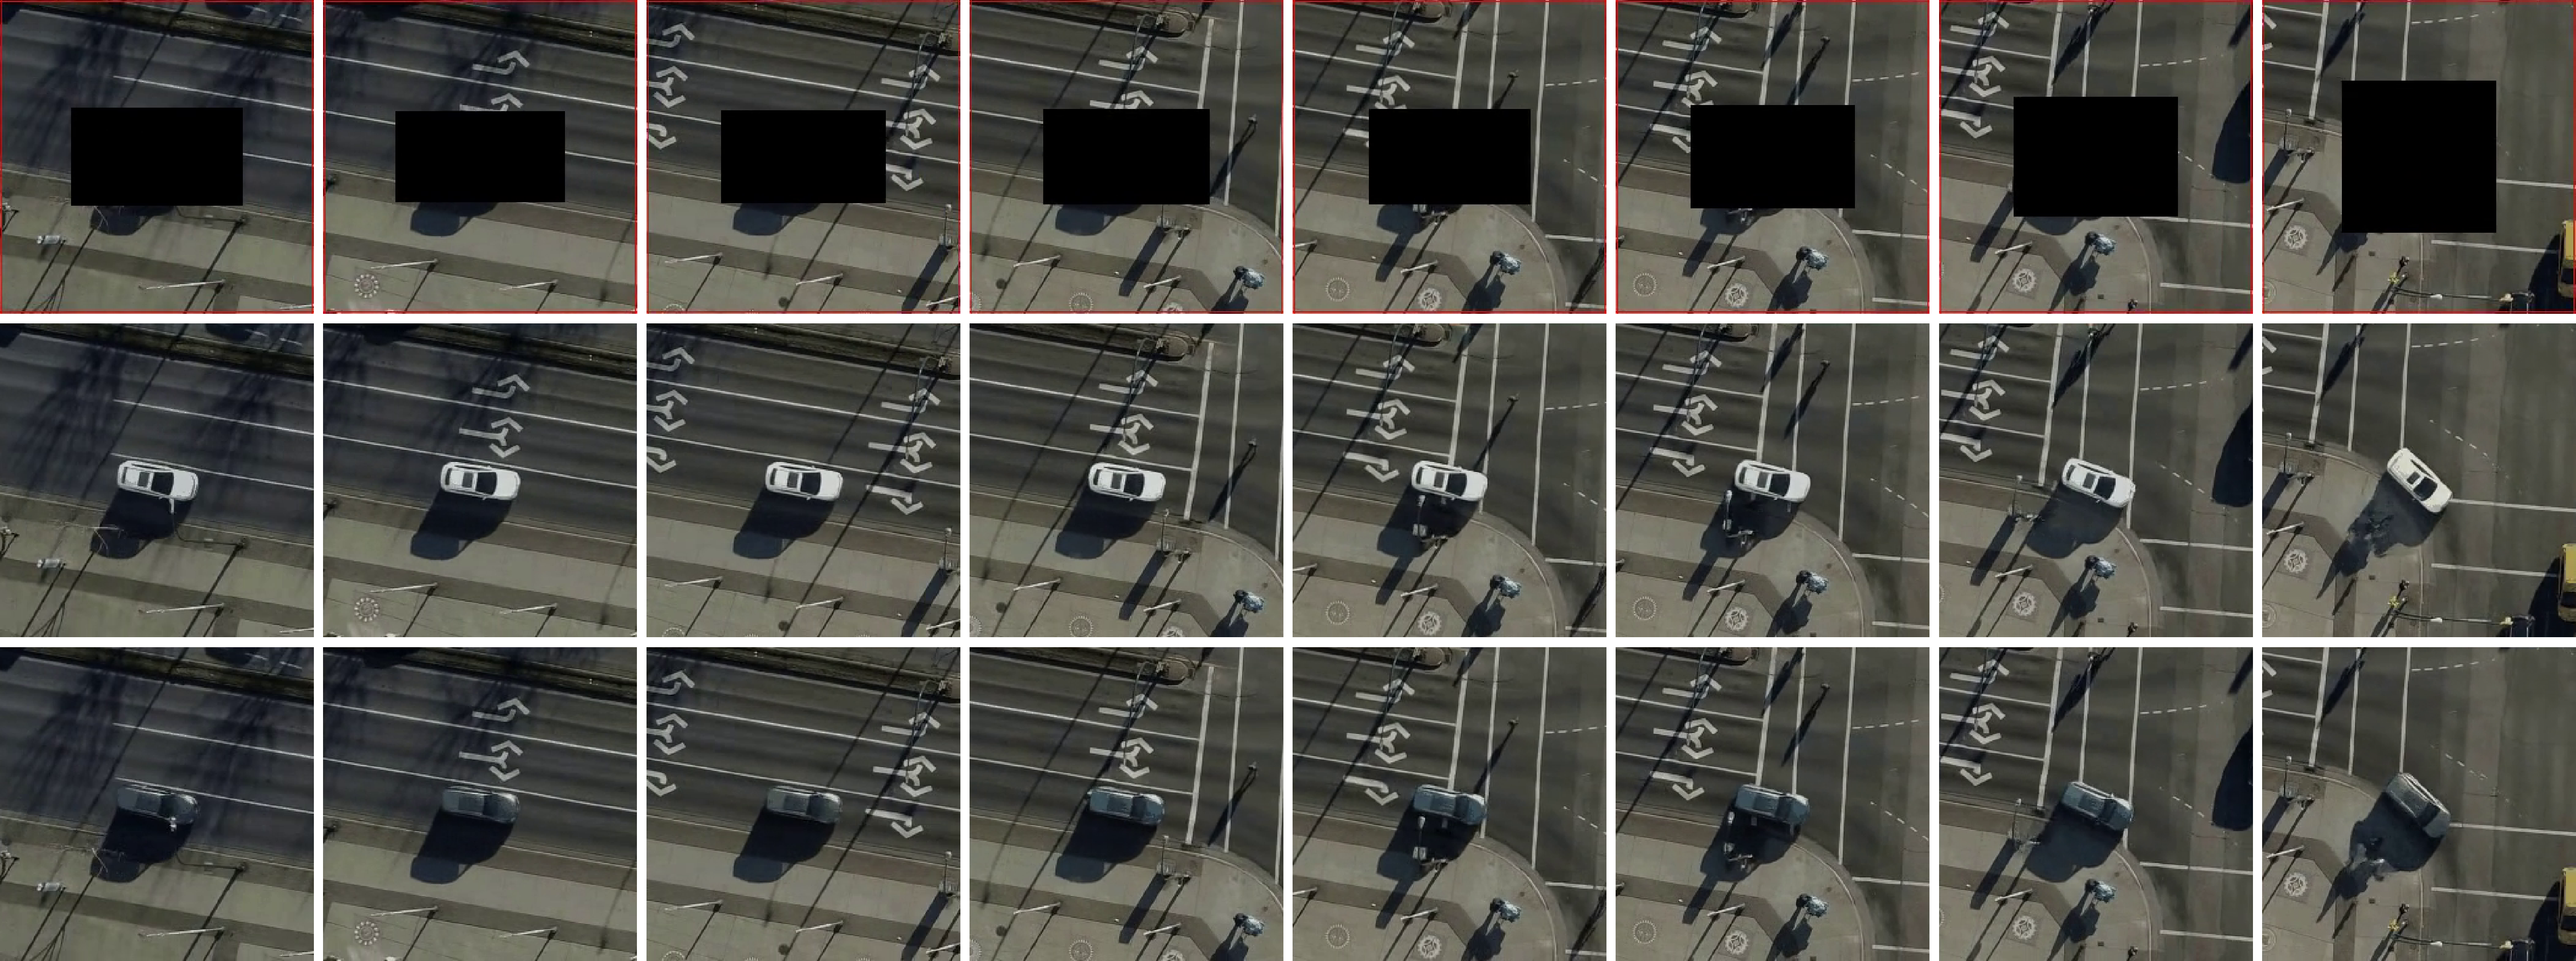
\includegraphics[width=\linewidth]{figures/updated-cars.pdf}
    \captionof{figure}{Inpaintings from our model on the Inpainting-Cars dataset. The first row is the masked input to the model, the lower two rows are two separate inpaintings sampled from our model.}
    \label{fig:cars}
\end{center}%
\end{figure*}
\subsection{Inpainting-Cars}
Sampled inpaintings from our model on an example from the Inpainting-Cars dataset are shown in \cref{fig:cars}. Our model is capable of generating diverse, visually realistic inpaintings for a given input. We note the model's ability to use \emph{semantic} cues from the context to generate plausible visual features, such as realistic behavior of shadows and plausible turning trajectories based only on the movement of the mask.

\section{Ablations}

\subsection{Effect of Sampling Schemes}
We compare selected sampling schemes on the Traffic-Scenes dataset in \Cref{table:samplingschemes}, before providing more thorough qualitative and quantitative comparisons in the appendix. Improved AR w/ Far Future is the best on all datasets aside from Infilling-Background in terms of video realism (VFID) and temporal consistency (warp error), demonstrating the importance of our method's ability to condition on incomplete frames. AR tends to do poorly on all metrics on both the Traffic-Scenes and BDD-Inpainting datasets. This is likely due to its inability to account for observed pixel values in frames coming after the ones being generated at each stage, causing divergence from the ground-truth and then artifacts when producing later frames conditioned on incompatible values. Hierarchy-2 does well on some metrics of reconstruction and frame-wise perceptual quality. It does less well in terms of video realism, as the inpainting of the ``keyframes'' in the first stage is done without conditioning on the known pixels of frames in their immediate vicinity, potentially leading to incompatibility with the local context.
\begin{table}[t]
\centering
\caption{Effect of sampling schemes, measured on the Traffic-Scenes test set.}
\label{table:samplingschemes}
\customrescaleone{
\begin{tabular}{llllllllllllll}
\toprule
Sampling Scheme & PSNR$\blacktriangle$ & SSIM$\blacktriangle$   & LPIPS$\blacktriangledown$     & PVCS$\blacktriangledown$   & FID$\blacktriangledown$   & VFID$\blacktriangledown$   & $E_\text{warp}$$\blacktriangledown$ \\ 
\midrule
AR                 & 31.72 & 0.9595 & 0.0392 & 0.2989 & 8.85 & 0.3016 & $3.01{\cdot}10^{\shortminus4}$ \\
Hierarchy-2                    & \textbf{35.53} & \textbf{0.9794} & \textbf{0.0196} & 0.1732 & \textbf{4.55} & 0.1714 & $2.48{\cdot}10^{\shortminus4}$ \\
Improved AR w/ Far Future                 & 35.29 & 0.9783 & 0.0202 & \textbf{0.1725} & 4.87 & \textbf{0.1637} & $\mathbf{2.26{\cdot}10^{\shortminus4}}$ \\
3-Res. Improved AR & 35.32 & 0.9785 & 0.0210 & 0.1815 & 5.07 & 0.1821 & $2.43{\cdot}10^{\shortminus4}$ \\
\bottomrule
\end{tabular}}
\end{table}

\subsection{Samplers and Number of Sampling Steps}
The use of diffusion models allows for a trade-off of computation time \vs inpainting quality through the number of steps used in the generative process. In \Cref{table:samplingsteps} we report the results of our model on the BDD-Inpainting test set with the AR sampling scheme using different samplers and numbers of sampling steps. Aligning with expectations and qualitative observations, performance on metrics degrades as the number of sampling steps decreases for LPIPS, PVCS, FID and VFID. We note, however, that performance on $E_\text{warp}$, PSNR, and SSIM improves, suggesting that these metrics may not correlate well with perceived quality, as has been previously suggested for the latter two metrics in \citet{perceptual}.
\begin{table}[t]
\centering
\caption{Effect of diffusion samplers, using AR sampling on BDD-Inpainting.}
\label{table:samplingsteps}
\customrescaleone{
\begin{tabular}{llllllllllllll}
\toprule
Sampler & PSNR$\blacktriangle$ & SSIM$\blacktriangle$   & LPIPS$\blacktriangledown$     & PVCS$\blacktriangledown$   & FID$\blacktriangledown$   & VFID$\blacktriangledown$   & $E_\text{warp}$$\blacktriangledown$ \\ 
\midrule
Heun (10 steps)   & 33.00  & 0.9687 & 0.0339 & 0.2437 & 2.39  & 0.1155 & $\mathbf{1.66{\cdot}10^{\shortminus3}}$            \\
Heun (25 steps)   & \textbf{33.05}  & \textbf{0.9703} & 0.0290 & 0.2202 & 1.84  & 0.0815 & $1.78{\cdot}10^{\shortminus3}$            \\
Heun (50 steps)   & 33.00  & 0.9699 & 0.0282 & 0.2177 & 1.81  & \textbf{0.0766} & $1.82{\cdot}10^{\shortminus3}$            \\
Heun (100 steps)  & 32.98  & 0.9700 & 0.0280 & \textbf{0.2171} & 1.76  & 0.0788 & $1.85{\cdot}10^{\shortminus3}$            \\
DDPM (1000 steps) & 32.41  & 0.9665 & \textbf{0.0272} & 0.2244 & \textbf{1.68}  & 0.0779 & $2.39{\cdot}10^{\shortminus3}$            \\
\bottomrule
\end{tabular}}
\end{table}


\chapter{Conclusion}
In this work, we have presented a framework for video inpainting by conditioning video diffusion models. This framework allows for flexible conditioning on the context, enabling post-hoc experimentation with sampling schemes which can greatly improve results. We introduce four challenging tasks for video inpainting methods and demonstrate our model's ability to use semantic information in the context to solve these tasks effectively. Our experiments demonstrate a clear improvement on quantitative metrics and, contrary to existing methods, our approach can generate semantically meaningful completions based on minimal information in the context.

%\subsubsection{Acknowledgements} We acknowledge the support of the Natural Sciences and Engineering Research Council of Canada (NSERC), the Canada CIFAR AI Chairs Program, Inverted AI, MITACS, the Department of Energy through Lawrence Berkeley National Laboratory, and Google. This research was enabled in part by technical support and computational resources provided by the Digital Research Alliance of Canada Compute Canada (alliancecan.ca), the Advanced Research Computing at the University of British Columbia (arc.ubc.ca), and Amazon.

%    2. Main body
% Generally recommended to put each chapter into a separate file
%\include{relatedwork}
%\include{model}
%\include{impl}
%\include{discussion}
%\include{conclusions}

%    3. Notes
%    4. Footnotes

%    5. Bibliography
\begin{singlespace}
\raggedright
\bibliographystyle{abbrvnat}
\bibliography{egbib}
\end{singlespace}

\appendix
%    6. Appendices (including copies of all required UBC Research
%       Ethics Board's Certificates of Approval)
%\include{reb-coa}	% pdfpages is useful here
%\chapter*{Supplementary Materials}
%\chapter{Limitations}
The most notable limitation of our method is its computational cost relative to competing methods. The wall-clock time for our method is highly dependent on a number of factors, such as the number of sampler steps used and the number of frames generated in each stage of the sampling scheme used. Improvements in few-step generation for diffusion models and increasing the size of our model such that more frames can be processed at a time would both help to mitigate these concerns. Additionally, our method requires that a model be trained on a specific dataset which is reasonably close to the data distribution to be inpainted at test time, requiring large datasets. The development of large scale, general purpose video generative models would likely help to make generative approaches such as ours more robust to out-of-distribution tasks.  

%\chapter{Potential Negative Impacts}
The development of generative models for the generation of photo-realistic video opens the door to malicious or otherwise unethical uses which could have negative impacts on society. While our method is currently limited to operating on data which is sufficiently similar to the datasets it was trained on, and those datasets have limited potential for malicious use, future work which takes a generative approach to video inpainting could be used for the purposes of misinformation, harassment or deception. 
\chapter{Dataset Creation Details}
\label{app:datasetss}
\section{BDD-Inpainting}

From the original BDD100K dataset we take a random subset of videos, using 48,886 for a training set and 100 for each held-out test set. Videos are downsampled spatially by a factor of 2.5, center-cropped to $256 \times 256$, and the frame rate is reduced by a factor of three to 10 fps.  We truncate videos to 400 frames, corresponding to a 40 second length for each. We randomly generate a set of 49,970 masks of four types: grids, horizontal or vertical lines, boxes, and blobs. Our mask generation procedure first picks a mask type, and then randomly selects mask parameters such as size and direction of motion (which includes stationary masks). Generated masks contain 400 frames. During training both videos and masks are sampled uniformly and independently, giving a distribution over nearly 2.5 billion video-mask pairs. Our test sets, as well as code for regenerating our training set, will be made public upon publication.

\section{Inpainting-Cars}
 We use an in-house dataset of overhead drone footage of vehicle traffic, for which we have tracker-generated bounding boxes for each vehicle. The videos are spatially downsampled by a factor of two from their original 4k resolution, and  $256 \times 256$ sub-videos centred on vehicles are extracted using the vehicle-specific tracks. The length of these videos is variable as it depends on the amount of time a given vehicle was visible in the source video, but typically ranges from 10 to 60 seconds at 10 fps. Bounding boxes are dilated by a factor of two to ensure the entirety of the vehicle is contained within them, and these dilated bounding boxes are then used as masks. This dataset contains 2973 training examples and 100 held-out test examples. 

\section{Inpainting-Background}
 The process for creating the Inpainting-Background is nearly identical to that of Inpainting-Cars. The primary difference is that the tracks are shifted in time to find new tracks which do not intersect with the bounding box of any other vehicle, giving a dataset where the masked out region contains the road surface and other environmental factors. Beyond that, videos are processed in the same way and are of the same length as those in Inpainting-Cars. This dataset contains 2965 training examples and 100 held-out test examples.  

 \section{Traffic Scenes}
This dataset is created using the same in-house dataset as was used for Inpainting-Cars and Inpainting-Background. The 4k, 10 fps source videos are spatially downsampled by a factor of 7.25, truncated to 200 frames and cropped to $256 \times 256$, with the crops centred over road features like intersections, roundabouts, highway on-ramps, \etc. We generate masks using the same mask generation procedure as in BDD-Inpainting. 


\chapter{Training Details}

All models are trained with 4 $\times$ NVIDIA A100 GPUS with a batch size of one, corresponding to an effective batch size of 4 as gradients are aggregated across GPUs. 
All models were trained to condition on or generate 16 frames at a time, use an EMA rate of 0.999, and use the AdamW \citep{AdamW} optimizer. We use the noise schedules defined in \citet{noiseschedules}: \texttt{linear} for the Inpainting-Background model, \texttt{cosine} for Inpainting-Cars, and \texttt{sigmoid} for BDD-Inpainting and Traffic-Scenes. All models use temporal attention at the spatial resolutions (32, 16, 8) in the U-Net, except for the Inpainting-Cars model where temporal attention only occurs at resolutions (16, 8). Otherwise, the default hyperparameters from our training code are used for all models. This code, and the BDD-Inpainting checkpoint, will be released upon publication. The number of training iterations for each model is listed below:
\begin{table}[h!]
\centering
\begin{tabular}{lc}
\toprule
Dataset               & Iterations (millions) \\ 
\midrule
BDD-Inpainting        & 2.5                   \\
Inpainting-Cars       & 1.1                   \\
Inpainting-Background & 1.5                   \\
Traffic-Scenes        & 2.4                  \\
\bottomrule
\end{tabular}
\end{table}





\chapter{Additional Ablations}
\section{Additional Sampling Scheme Ablations}
\Cref{table:samplingschemesnotblobs} and \Cref{table:samplingschemesblobs} show the effect of using different sampling schemes on the BDD-Inpainting and BDD-Inpainting-Blobs test sets, respectively. The sampling schemes tested are depicted in \cref{fig:old-sampling-schemes} and \cref{fig:sampling-schemes}. For each metric, the best performing sampling scheme is indicated in bold font. All measurements were taken using the Heun sampler \cite{karras2022elucidating} with 100 sampling steps. The Improved AR w/ Far Future performs best on both test sets across almost all metrics. Sampling scheme ablations are omitted for Inpainting-Background and Inpainting-Cars as we found an autoregressive scheme gave significantly better qualitative results than the other schemes.
\begin{table}[h]
\centering
\caption{Effect of sampling schemes measured on the BDD-Inpainting test set.}
\label{table:samplingschemesnotblobs}
\customrescaleone{
\begin{tabular}{llllllllllllll}
\toprule
Sampling Scheme & PSNR$\blacktriangle$ & SSIM$\blacktriangle$   & LPIPS$\blacktriangledown$     & PVCS$\blacktriangledown$   & FID$\blacktriangledown$   & VFID$\blacktriangledown$   & $E_\text{warp}$$\blacktriangledown$ \\ 
\midrule
3-Res. Improved AR                                                & 32.81 & 0.9678 & 0.0289 & 0.2302 & 1.75 & 0.0884 & $2.19{\cdot}10^{\shortminus3}$ \\
Improved AR w/ Far Future                                         & 33.68 & \textbf{0.9717} & \textbf{0.0261} & \textbf{0.2037} & \textbf{1.71} & \textbf{0.0748} & $\mathbf{1.79{\cdot}10^{\shortminus3}}$ \\
AR                                                                & 32.97 & 0.9699 & 0.0278 & 0.2166 & 1.78 & 0.0778 & $1.85{\cdot}10^{\shortminus3}$ \\
Hierarchy-2                                                       & 32.96 & 0.9690 & 0.0284 & 0.2232 & 1.74 & 0.0839 & $1.97{\cdot}10^{\shortminus3}$ \\
2-Res. Improved AR                                                & 33.18 & 0.9692 & 0.0278 & 0.2201 & 1.72 & 0.0815 & $2.03{\cdot}10^{\shortminus3}$ \\
Reverse AR                                                        & \textbf{33.31} & 0.9702 & 0.0273 & 0.2132 & 1.76 & 0.0785 & $\mathbf{1.79{\cdot}10^{\shortminus3}}$ \\ 
\bottomrule
\end{tabular}}
\end{table}
\begin{table}[h]
\centering
\caption{Effect of sampling schemes measured on the BDD-Inpainting-Blobs test set.}
\label{table:samplingschemesblobs}
\customrescaleone{
\begin{tabular}{llllllllllllll}
\toprule
Sampling Scheme & PSNR$\blacktriangle$ & SSIM$\blacktriangle$   & LPIPS$\blacktriangledown$     & PVCS$\blacktriangledown$   & FID$\blacktriangledown$   & VFID$\blacktriangledown$   & $E_\text{warp}$$\blacktriangledown$ \\ 
\midrule
3-Res. Improved AR                        & 29.89 & 0.9561 & 0.0475 & 0.3142 & 1.63 & 0.1188 &  $2.00{\cdot}10^{\shortminus3}$ \\
Improved AR w/ Far Future                 & \textbf{30.67} & \textbf{0.9608} & \textbf{0.0442} & \textbf{0.2857} & 1.69 & \textbf{0.1083} &  $1.53{\cdot}10^{\shortminus3}$  \\
AR                                        & 29.45 & 0.9547 & 0.0512 & 0.3319 & 2.07 & 0.1328 &  $1.61{\cdot}10^{\shortminus3}$  \\
Hierarchy-2                               & 29.97 & 0.9570 & 0.0474 & 0.3106 & 1.65 & 0.1137 &  $1.74{\cdot}10^{\shortminus3}$  \\
2-Res. Improved AR                        & 30.25 & 0.9583 & 0.0454 & 0.2991 & \textbf{1.59} & 0.1116 &  $1.79{\cdot}10^{\shortminus3}$   \\
Reverse AR                                & 30.04 & 0.9590 & 0.0450 & 0.2920 & 1.8  & 0.1134 &  $\mathbf{1.51{\cdot}10^{\shortminus3}}$  \\
\bottomrule
\end{tabular}}
\end{table}
\section{Qualitative Sampling Scheme Ablations}
\label{sec:quall}
In this section we highlight the qualitative impact that different sampling schemes can have on the quality of inpainted videos. We select a video from the test set where conditioning on the appropriate frames is crucial for our method to succeed. \Cref{fig:qual-begin} shows the beginning of this video, where a car is occluded in the right-hand lane for the first few seconds of the video (see input frames in the first row). The Autoregressive scheme (second row) shows a distinct ``pop-in'' effect, as when the initial frames were generated the model was not able to condition on future frames where the cars existence and appearance are revealed. Both Reverse-Autoregressive and AR w/ Far Future (third and fourth rows) do condition on future frames that contain the car; Reverse-Autoregressive because the model is able to propagate the car backwards through time, and AR w/ Far Future because the model conditions on frames far out into the future where the car has been revealed. \Cref{fig:qual-end} shows the end of the video, where the cars in the right-hand lane are occluded and remain occluded for the rest of the video (first row). The Autoregressive scheme keeps these cars visible, as it is able to propagate them forward through time (second row). Reverse-Autoreg (third row) fails for the same reason that Autoreg did at the beginning: when the final frames were generated, the model was not able to condition on frames where the vehicles were visible. AR w/ Far Future (fourth row) is again successful; despite the cars not becoming visble again (and thus there is no ``future'' to condition on), it is able to propagate the cars forward in time as the Autoreg scheme does. We provide an mp4 video showing the entire inpainting for this video using the sampling schemes discussed here and more in the supplementary, with filename \texttt{appendix\_E2.mp4}. Sampling schemes used in each tile are labelled in the video.
\begin{figure*}[h!]
\begin{center}
    \centering
    \captionsetup{type=figure}
    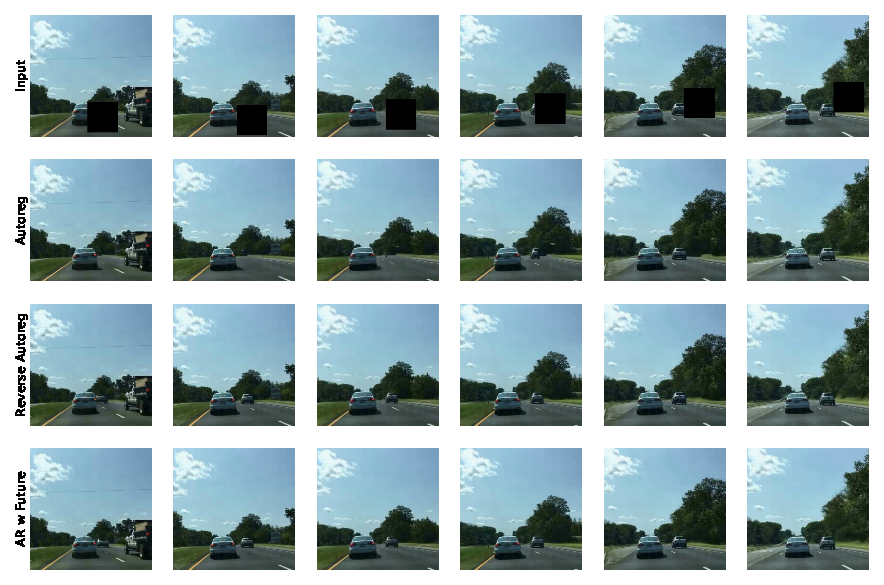
\includegraphics[width=\linewidth]{figures/james_quall/james_quall_beginning.pdf}
    \caption{Qualitative results from different sampling schemes on the beginning of the video discussed in \cref{sec:quall}}
    \label{fig:qual-begin}
    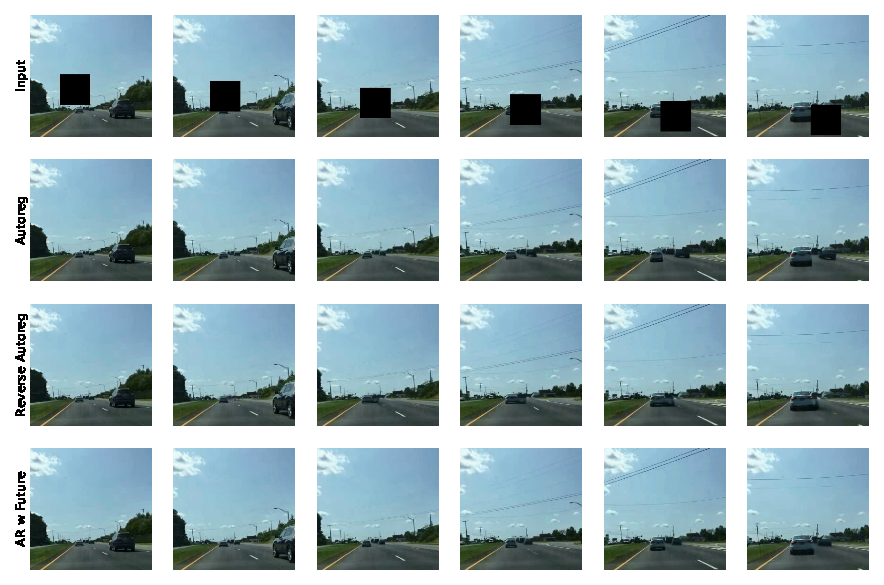
\includegraphics[width=\linewidth]{figures/james_quall/james_quall_end.pdf}
    \caption{Qualitative results from different sampling schemes on the end of the video discussed in \cref{sec:quall}}
    \label{fig:qual-end}
\end{center}
\end{figure*}







%\section{Algorithms}
\hlr{UPDATE TO DEAL WITH Z}

\begin{algorithm}[h]
\caption{Training}
\label{alg:train}
\begin{algorithmic}[1]
\Repeat
\State $(\bV, \bM) \sim q(\bV, \bM)$\Comment{Sample video and mask}
\State $(\mathcal{X}, \mathcal{Y}) \sim u(\mathcal{X}, \mathcal{Y})$\Comment{Sample training task}
\State $t \sim \mathcal{U}(\{1 \ldots T\})$
\State $\boldsymbol{\epsilon} \sim \mathcal{N}(\mathbf{0}, \mathbf{I})$
\State $(\bV', \bM') \gets (\bV[\fX \cup \fY], \bM[\fX \cup \fY])$\Comment{Extract selected frames}
\State $\bV_t' \gets \sqrt{\bar{\alpha}_t}\bV' + \sqrt{1-\bar{\alpha}_t}(\mathbbm{1}-\bM')\odot\boldsymbol{\epsilon}$\Comment{Noise latent pixels}
\State Take gradient descent step on \newline
\hspace*{3em}$\nabla_\theta \|(1-\bM')\odot(\boldsymbol{\epsilon} - \boldsymbol{\epsilon}_\theta(\bV_t', \bM', \mathcal{X}, \mathcal{Y}, t))\|^2$\Comment{Masked loss}
\Until converged
\end{algorithmic}
\end{algorithm}

\begin{algorithm}[h]
\caption{Inpaint video $\bV$ given mask $\bM$ and sampling scheme $\left[(\mathcal{X}_s, \mathcal{Y}_s)\right]^S_{s=1}$}
\label{alg:alg}
\begin{algorithmic}[1]
\For{$s \gets 1, \ldots, S$}
\State $\bV_s' \gets \bV [\fX_s \cup \fY_s]$\Comment{Extract selected video frames}
\State $\bM_s' \gets \bM [\fX_s \cup \fY_s]$\Comment{Extract selected mask frames}
\State $\hat{\bV}_s \sim \texttt{DDPM}(\cdot;\bV_s', \bM_s', \mathcal{X}, \mathcal{Y},\theta)$\Comment{Sample}
\State $\bV [\fX_s \cup \fY_s] \gets \hat{\bV}_s$\Comment{Insert completed frames}
\State $\bM [\fX_s] \gets \mathbbm{1}$\Comment{Update masks for inpainted frames}
\EndFor
\State \Return $\bV$
\end{algorithmic}
\end{algorithm}
\chapter{Diffusion Model Sampling Details}
As alluded to in the main paper, we train a diffusion model that uses $\epsilon$-prediction to parameterize the score of a distribution over $\bx_t$ at each time $t$. This can be used to parameterize a stochastic differential equation (or ordinary differential equation) that morphs samples from a unit Gaussian into approximate samples from the conditional distribution of interest $p_\text{data}(\bx|\by)$ \citep{song2020score}. We use the Heun sampler proposed by \citet{karras2022elucidating} to integrate this SDE. Our hyperparameters are $\sigma_\text{max}=1000$, $\sigma_\text{min} = 0.002$, $\rho=7$, $S_\text{churn}=80$, $S_\text{max}=\infty$, $S_0=0$, and $S_\text{noise}=1$. We use 100 sampling steps (involving 199 network function evaluations) for each experiment except where specified otherwise. 









\backmatter
%    7. Index
% See the makeindex package: the following page provides a quick overview
% <http://www.image.ufl.edu/help/latex/latex_indexes.shtml>


\end{document}
